% Autor: Leonhard Segger, Alexander Neuwirth
% Datum: 2017-10-30
\documentclass[
	% Papierformat
	a4paper,
	% Schriftgröße (beliebige Größen mit „fontsize=Xpt“)
	12pt,
	% Schreibt die Papiergröße korrekt ins Ausgabedokument
	pagesize,
	% Sprache für z.B. Babel
	ngerman
]{scrartcl}

% Achtung: Die Reihenfolge der Pakete kann (leider) wichtig sein!
% Insbesondere sollten (so wie hier) babel, fontenc und inputenc (in dieser
% Reihenfolge) als Erstes und hyperref und cleveref (Reihenfolge auch hier
% beachten) als Letztes geladen werden!

\usepackage{tikz}
\usetikzlibrary{calc,patterns,angles,quotes} % loads some tikz extensions\usepackage{tikz}
\usetikzlibrary{babel}

% Silbentrennung etc.; Sprache wird durch Option bei \documentclass festgelegt
\usepackage{babel}
% Verwendung der Zeichentabelle T1 (Sonderzeichen etc.)
\usepackage[T1]{fontenc}
% Legt die Zeichenkodierung der Eingabedatei fest, z.B. UTF-8
\usepackage[utf8]{inputenc}
% Schriftart
\usepackage{lmodern}
% Zusätzliche Sonderzeichen
\usepackage{textcomp}

% Mathepaket (intlimits: Grenzen über/unter Integralzeichen)
\usepackage[intlimits]{amsmath}
% Ermöglicht die Nutzung von \SI{Zahl}{Einheit} u.a.
\usepackage{amssymb}
% mehr symbole plox
\usepackage{siunitx}
% Zum flexiblen Einbinden von Grafiken (\includegraphics)
\usepackage{graphicx}
% Abbildungen im Fließtext
\usepackage{wrapfig}
% Abbildungen nebeneinander (subfigure, subtable)
\usepackage{subcaption}
% Funktionen für Anführungszeichen
\usepackage{csquotes}
\MakeOuterQuote{"}
% Zitieren, Bibliografie
\usepackage[sorting=none]{biblatex}


% Zur Darstellung von Webadressen
\usepackage{url}
%chemische Formeln
\usepackage[version=4]{mhchem}
% siunitx: Deutsche Ausgabe, Messfehler getrennt mit ± ausgeben
\usepackage{floatrow}
\floatsetup[table]{capposition=top}
\usepackage{float}
% Verlinkt Textstellen im PDF-Dokument
\usepackage[unicode]{hyperref}
% "Schlaue" Referenzen (nach hyperref laden!)
\usepackage{cleveref}
\sisetup{
	locale=DE,
	separate-uncertainty
}
\bibliography{BA-C-04_SLM_27-05-2019_References}

\begin{document}

	\begin{titlepage}
		\centering
		{\scshape\LARGE Versuchsbericht zu \par}
		\vspace{1cm}
		{\scshape\huge Räumlicher LC-Modulator und diffraktive Optik \par}
		\vspace{2.5cm}
		{\LARGE Gruppe BA-C-04 \par}
		\vspace{0.5cm}

		{\large Alexander Neuwirth (E-Mail: a\_neuw01@wwu.de) \par}
		{\large Leonhard Segger (E-Mail: l\_segg03@uni-muenster.de) \par}
		\vfill

		durchgeführt am 27.05.2019\par
		betreut von\par
		{\large Milena Merkel}

		\vfill

		{\large \today\par}
	\end{titlepage}
	\tableofcontents
	\newpage

	\section{Kurzfassung}
	% Hypothese	und deren Ergebnis, wenn Hypothese ist, dass nur Theorie erfüllt, sagen: Erwartung: Theorie aus einführung (mit reflink) erfüllt
	% Ergebnisse, auch Zahlen, mindestens wenn's halbwegs Sinn ergibt
	% Was wurde gemacht
	% manche leute wollen Passiv oder "man", manche nicht
	In diesem Versuch wird ein Modulator aus Flüssigkristallzellen verwendet, um dessen Eigenschaften zu untersuchen und seine Verwendbarkeit als verschiedene diffraktive optische Elemente zu zeigen.
	Zunächst kann dabei das Gesetz von Malus bestätigt werden und gezeigt und erklärt werden, dass bzw. warum der Kontrast des LC-Modulators von der Eingangspolarisation abhängt.
	Für den verwendeten LC-Modulator wird mit zwei verschiedenen Methoden der Pixelabstand bestimmt und der Füllfaktor der Zellen wird abgeschätzt.
	Außerdem wird die Abhängigkeit der Ausgangspolarisation des Modulators von dem eingestellten Grauwert untersucht und diskutiert.

	Es werden Beugungsbilder des LC-Modulator als verschiedene diffraktive optische Elemente aufgenommen, um zu zeigen, dass der LC-Modulator als solche verwendet werden kann.
	Bei Verwendung des LC-Modulators als Fresnel-Linse wird gezeigt, dass er auch eine Linse variabler Brennweite darstellen kann.

	Zuletzt werden Fouriertransformierte von simplen Bilder auf den LC-Modulator gegeben, um mit seiner Hilfe Hologramme auf dem Kamerasensor zu erzeugen.

  \section{Theorie}
	% wdh. Texte
	% wdh. Besprechung

	\subsection{Gesetz von Malus}

	Nach dem Gesetz von Malus verhält sich die Intensität von linear polarisiertem Licht, nachdem es einen idealen Polarisationsfilter passiert hat, folgendermaßen in Abhängigkeit vom Winkel $\alpha $ zwischen Polarisationsfilterrichtung und Polarisationsrichtung der Welle:

	\begin{equation}
		I = I_0 \cos ^2(\alpha)
	\end{equation}

	\subsection{Flüssigkristallzellen}
	% ist ultra von dem anderen Versuch gecopypasted, aber das sollte ja wohl erlaubt sein.
	% vlt mal in das alte Protokoll (MP5) schauen (kp, ob der das als pdf oder ausgedruckt wiedergegeben hat) und schauen, ob hier irgendwas falsch war.

	Flüssigkristalle zeichnen sich dadurch aus, dass sie mindestens unter bestimmten Bedingungen eine Orientierungsfernordnung, aber keine vollständige Positionsfernordnung, aufweisen, womit sie sich in letzterem Punkt von \enquote{gewöhnlichen} Kristallen unterscheiden.
	Positionsfernordnung bezeichnet hierbei eine Anordnung im Raum, die sich durch das periodische Fortsetzen einer Einheitszelle beschreiben lässt.
	Eine unvollständige Positionsfernordnung meint eine Periodizität in nur einer oder nur zwei Dimensionen.
	Orientierungsfernordnung meint, dass eine Vorzugsrichtung der Längsachsen der Moleküle des Flüssigkristalls existiert.
	Diese ist periodisch ortsabhängig oder konstant.
	Der Grad der Ordnung lässt sich als die Größe der durchschnittlichen Abweichung von der Vorzugsrichtung verstehen.

	Für die Herstellung von Flüssigkristallanzeigen wird ein Flüssigkristall in cholesterischer Phase verwendet. % hier stand in der Anleitung immer "twisted nematic". Denke, das ist das gleiche.
	Dies meint, dass die Molekülachsen ebenenweise in die gleiche Richtung zeigen.
	Die Orientierung in den Ebenen ist dabei periodisch, da der Direktor (die Vorzugsachse) sich, wenn in Laufrichtung senkrecht zur Ebene betrachtet, mit konstanter Winkelgeschwindigkeit dreht und eine Helixstruktur bildet, wenn das Ende des Direktorvektors im Raum verfolgt wird.

	\begin{figure}[H]
			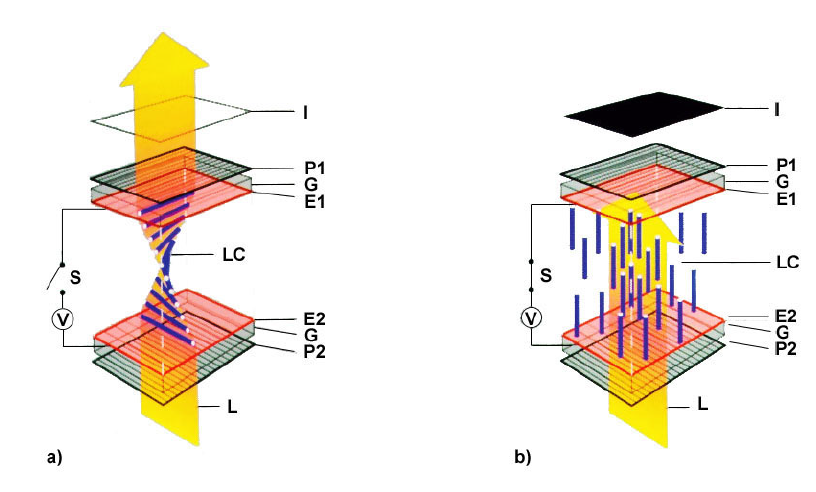
\includegraphics[width=1\linewidth]{img/displayHelix}
			\caption{
			Polarisationsrichtung in der Flüssigkristallanzeige. a) ohne angelegte Spannung. b) bei angelegter Spannung. E1, E2: Elektroden (ITO); G: Glasplatten; I: Lichtintensität; L: Lichtwelle; LC: Flüssigkristall;
P1, P2: Polarisatoren; S: Schalter, V: Spannungsquelle. \cite{displayHelix}
			}
			\label{fig_displayHelixBild}
	\end{figure}

	Dies erlaubt den Bau einer Flüssigkristallanzeige, da in einem Flüssigkristall in cholesterischer Mesophase die Polarisation des Lichtes, wenn es entlang besagter Laufrichtung einfällt, der Helixform des Direktors folgt.
	Wenn bekannt ist, mit welcher Ganghöhe (Länge der Helix bei einer Umdrehung des Direktors) der Kristall vorliegt, kann auf der Ausgangsseite des Displays linear polarisiertes Licht einen Polfilter passieren, wenn dieser zur Einfallsrichtung soweit gedreht ist, wie sich der Direktor über die Dicke des Flüssigkristalls im Display dreht.
	Häufig wird hierfür eine Vierteldrehung verwendet. Wie gleich deutlich wird, sind hier nur Drehungen um $\frac{\pi (2z+1)}{2}$ mit $z \in \mathbb{Z}$ praktikabel.
	Da für die lineare Polarisation des einfallenden Lichts ebenfalls ein Polfilter verwendet wird, ist eine solche Flüssigkristallanzeige bidirektional.
	Wenn jetzt im Flüssigkristall ein annähernd homogenes elektrisches Feld angelegt wird, richten sich die Molekülachsen statt nach der Helixstruktur mit zunehmender Feldstärke zunehmend eher nach dem Feld aus (vgl. \cref{fig_displayHelixBild}). % , wenn es sich bei diesem um Dipole handelt, aber sonst tut das eh nicht
	Dies verhindert, dass sich die Polarisation des Lichtes im Innern ändert, weshalb bei einer der oben genannten Drehungen zwischen den Durchlassrichtungen der Polarisationsfilter das Licht den zweiten Polarisationsfilter nicht passieren kann.
	Jetzt wird auch klar, warum nur die oben genannten Drehungen praktikabel sind:
	Die Polarisationsfilter müssen senkrecht zueinander stehen, damit im Falle von angelegter Spannung die Transmission minimal wird (vgl. Gesetz von Malus).

	Demnach ist eine spannungsgesteuerte Schaltung der Durchlässigkeit des Filters möglich und wenn hinter das Display eine Lichtquelle oder ein Spiegel gebracht wird, kann die Zelle als Pixel einer größeren Anzeige verwendet werden.
	Flüssigkristalldisplays werden mit Wechselspannung betrieben, da eine Gleichspannung die elektrolytische Zersetzung des Flüssigkristalls zufolge hätte. % wurde jetzt auch nirgendwo angesprochen.

	Beim im folgenden verwendeten LC-Modulator sind keine Polfilter in das Gerät eingebaut, weshalb polarisiertes Licht aus einem Laser verwendet wird und nach dem Modulator ein externer Polarisationsfilter verwendet wird.

\subsection{Doppelbrechung}
% sie meinte, dass dies für die Polarisationsänderung in der Helix verantwortlich wäre. Sehe ich nicht so recht. sollte man aber erwähnen, wenn es true ist. ergibt sich irgendwie in dem Abschnitt 1.1.3 wegen der Jones-Rechnung.

	Flüssigkristalle weisen einen polarisationsabhängigen Brechungsindex auf, da die Molekülelektronen je nach Orientierung der Moleküle und Schwingungsrichtung sich gegenseitig unterschiedlich stark zum Schwingen anregen.
	Dies führt bei einem Strahl, der nicht bereits entweder senkrecht oder parallel zur optischen Achse polarisiert ist, zum Phänomen der Doppelbrechung.
	Der Strahl spaltet in zwei senkrecht zueinander polarisierte Strahlen auf.
	Diese Aufspaltung wird maximal, wenn der einfallende Strahl senkrecht zum Direktor steht.
	%Wenn der Flüssigkristall in einem keilförmigen Gefäß ist, behält der Strahl nach dem Austritt aus dem Kristall eine Winkelaufspaltung, weshalb in größerem Abstand die Aufspaltung einfacher gemessen werden kann (vgl. \cref{fig_keil}).
	%In einem plan-parallelen Aufbau würden die Strahlen nach dem Austritt aus dem Kristall wieder parallel verlaufen und die Ortsaufspaltung würde nicht mit dem Messabstand steigen.
  %Die Differenz der Brechungsindizes ist dabei direkt abhängig vom Ordnungsgrad, weshalb sie als ein Maß für diesen verwendet werden kann.


	\subsection{Diffraktive Optische Elemente} %alles groß, weil Überschrift?
	% Jones-Vektoren, Jones-Formalismus?

	Mithilfe einer Matrix aus Flüssigkristallzellen lässt sich ein räumlicher Lichtmodulator realisieren.
	% 1.1.7 TN-LC-Zelle + Polarisator ergibt Amplitudenmodulation (und auch Phase)
	Polarisator, Mikrodisplay und Analysator sorgen in Kombination dafür, dass ein Phasenunterschied zwischen den Flüssigkristallzellen entsteht, der proportional zum eingestellten Grauwert ist.
	Dies ergibt sich aus der Betrachtung des Systems mittels des Jones-Formalismus.
	Durch einzelne Ansteuerung der Flüssigkristallzellen entsteht ein räumliche Lichtmodulation in Amplitude und Phase.
	\label{chap_phasengrau}
	% Interferenz?

	\subsection{Kohärenz}
	Der signifikante Unterschied zwischen einem Laser und einer Glimmlampe besteht in der Fähigkeit zur Interferenz.
	Die Lichtwellen, die den Laser verlassen haben eine feste Phasenbeziehung, weshalb nach Trennung des Strahls Interferenz zwischen beiden Teilstrahlen zu beobachten ist.

	Bei der qualitativen Beschreibung der Interferenzfähigkeit unterscheidet man zwischen räumlicher und zeitlicher Kohärenz.
	Zeitliche Kohärenz kann über Autokorrelation mittels des Michelson-Interferometers gemessen werden.
	Die Kohärenzlänge ist definiert durch den Abstand (optische Wegdifferenz), der die Länge eines Arms des Interferometers vom Interferenzmaximum wegbewegt werden kann, bevor die durch die Interferenz erzeugte Autokorrelationsfunktion nicht mehr über $1/\text{e}$ steigt.
	Die Kohärenzlänge ergibt sich aus der Monochromatizität des Lichts, da sich bei perfekt monochromatischem Licht die Phasenbeziehung über keine Entfernung ändert.
	Die räumliche Kohärenz kann mittels eines Doppelspaltexperiments (oder des Young-Interferometers) gemessen werden, da sie die Phasenbeziehung innerhalb einer Wellenfront beschreibt und der Doppelspalt Interferenz zwischen unterschiedlichen Teilen der Wellenfront realisiert.


	\subsection{Fraunhofer-Beugung}

	Was die Fraunhofer-Beugung angeht, reicht es sich hier darauf zu beschränken, dass durch die Beugung an diffraktiven optischen Elementen (DOEs) im Fernfeld eine Fouriertransformation des DOEs auftritt.
	Durch eine Linse kann diese Fouriertransformation rückgängig gemacht werden und das Bild wieder ins Nahfeld geholt werden.

	Räumliche Frequenzen tauchen im Beugungsbild also als Punkte auf.
	Einzelspalte entsprechen Rechteckfunktionen, die transformiert Funktionen der Form $\sin{x}/x$ ergeben.
	Bei einem Doppelspalt tauchen zusätzlich Nebenmaxima auf und bei Gittern ergeben sich einzelne Hauptmaxima hoher Intensität. %TODO confirmen.

	\section{Methoden}
	% Bilder von der Website klauen
	% einer will Präsens
	In \cref{fig_Aufbau} ist der Aufbau beispielhaft für einen der Versuchsschritte abgebildet.

	\begin{figure}[H]
				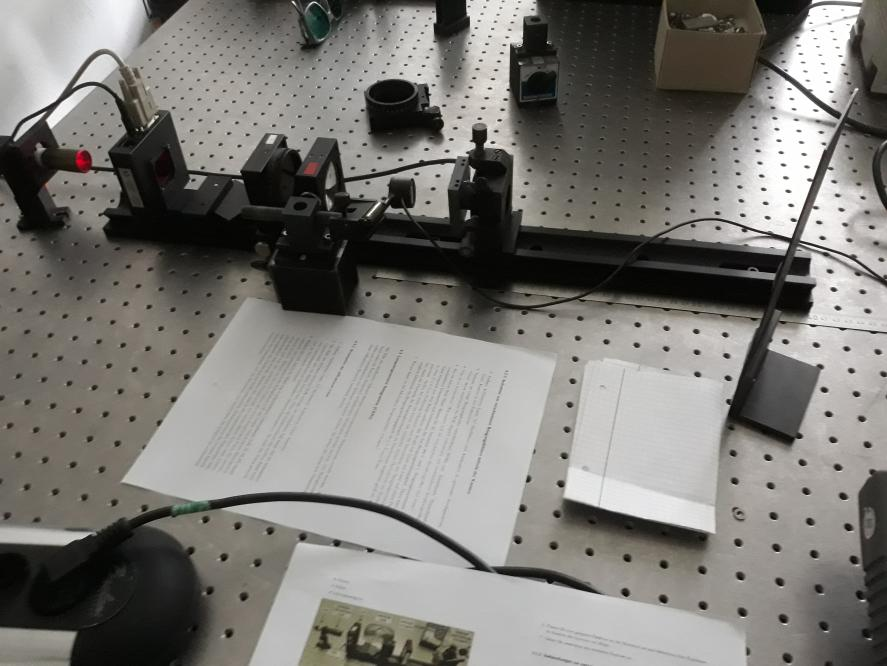
\includegraphics[width=0.7\linewidth]{img/aufbau}
				\caption{
				Fotografie des Aufbaus.
				}
				\label{fig_Aufbau}
		\end{figure}


	\subsection{Überprüfung des Gesetzes von Malus}
	Um das Gesetz von Malus zu überprüfen, wird das Licht eines He-Ne-Lasers durch einen Analysator geschickt und dann mit einer Linse auf ein Intensitätsmessgerät geschickt. % He-Ne können wir nicht confirmen, aber ist schon ziemlich safe.
	Hierbei wird vermutet, dass der Laser bereits linear polarisiertes Licht erzeugt.
	Der Analysator wird in \SI{10}{\degree}-Schritten um \SI{360}{\degree} rotiert.

	\subsection{Einstellung der Eingangspolarisation}
	Der im Folgenden verwendete LC-Modulator weist einen von der Eingangspolarisation abhängigen Kontrast auf.
	Der maximale Kontrast soll bei einer Eingangspolarisation von \SI{-45}{\degree} bzw. \SI{-135}{\degree} liegen.
	Um diese Eingangspolarisation zu erreichen wird ein Analysator in den Strahlengang gebracht und auf \SI{-135}{\degree} eingestellt.
	Dann wird der Laser rotiert, bis die gemessene Intensität maximal ist.
	Sobald diese Position gefunden ist, wird zwischen Laser und Analysator der LC-Modulator eingebaut, der Strahl kollimiert und mit einer Kamera das sich ergebende Bild aufgenommen.
	Auf dem LC-Modulator wird ein horizontal geteiltes Bild eingestellt (eine Hälfte Weiß, eine Schwarz).
	Dies wird im Folgenden als \textit{Horizontally Divided Screen} bezeichnet.
	Dann wird der Analysator um je \SI{90}{\degree} gedreht und jeweils ein Kamerabild aufgenommen, um zu zeigen, dass bei der gewählten Eingangspolarisation der Kontrast tatsächlich maximal ist. % man sollte hier streng genommen bei einem Winkel von 90deg ein invertiertes Bild verwenden. not sure why, haben wir aber nicht gemacht. -> Vermutlich, damit sich die Seiten nicht tauschen, aber schadet ja nicht, wenn sie es tun.

	Zusätzlich wird der Kontrast gemessen, indem ein komplett weißes bzw. schwarzes Bild (\textit{Blanc Screen}) verwendet wird und mit einem Intensitätsmessgerät nach Fokussierung durch eine Linse die Intensität in der Fokusebene gemessen wird.

	\subsection{Bestimmung der Pixelgröße}
		\subsubsection*{Variante 1}
		Um die Pixelgröße des LC-Modulators zu bestimmen, wird ein weißes Bild mit einem 200x200 Pixel großen schwarzen Quadrat in der Mitte auf den Modulator gegeben.
		Der Laserstrahl wird kollimiert.
		In den Strahlengang wird der LC-Modulator und im Abstand der Brennweite eine Linse dahinter gestellt, hinter der wieder im Abstand der Brennweite ein Schirm aufgestellt wird.
		Auf dem Schirm wird die Größe des Quadrats mit einem Lineal gemessen. % waren wir hier wirklich nicht mit dem Modulator im Fokus? Hatten wir hier überhaupt einen Polarisator, an dem wir hätten falsch messen können? -> kp und ja.
		\subsubsection*{Variante 2}
		Da die Pixel des LC-Modulators elektronische Strukturen zur Ansteuerung benötigen, bilden sie ein periodisches Gitter. %TODO sagte sie nicht noch irgendwas, woraus die Pixel bestehen würden?
		Aufgrund dessen ergibt sich in der Fokusebene das Beugungsbild eines Gitters.
		Es wird der Abstand zweier höherer Ordnungen mit einem Lineal gemessen und hieraus Gitterkonstante und somit Pixelgröße bestimmt.


	\subsection{Zusammenhang zwischen Grauwert und Polarisationszustand}

		Es wird auf dem LC-Modulator ein einfarbiges Bild angezeigt. % streng genommen Weiß/Schwarz keine Farben, wenn man pedantisch ist...
		In der Fokusebene wird die Intensität gemessen und bei sechs verschiedenen Grauwerten des Bildes jeweils das Maximum der Intensität in Abhängigkeit vom Analysatorwinkel gesucht.
		Da für die Bestimmung der Exzentrizität des Lichts auch die Intensität bei einem dazu um \SI{90}{\degree} gedrehten Analysators bekannt sein müsste, dies aber nicht gemessen wurde, werden hierfür im folgenden Daten aus \cite{JTZ} verwendet.

	\subsection{Intensitätsverteilung in den Beugungsordnungen des unadressierten Displays} % hier habe ich jetzt komplett den Titel übernommen
	Die Linse wird entfernt und stattdessen der Laser mittels der Linse am Laser auf einen Abstand von etwa \SI{90}{\centi \meter} fokussiert.
	Es wird in horizontaler und vertikaler Richtung die Intensität der ersten elf Ordnungen gemessen. % hier haben wir halt horziontal weniger. kp, ob man das hier oder unten erwähnen sollten.

	\subsection{Beugungsbilder verschiedener DOEs}
		Der Laser wird wieder kollimiert und eine Linse nach dem Analysator zur Fokussierung verwendet.
		Es wird nacheinander ein Einzelspalt, zwei verschiedene Doppelspalte und ein Gitter als DOE für den LC-Modulator eingestellt.
		Dann wird mit einer Kamera in der Fokusebene jeweils das Beugungsbild aufgenommen.
		Für ein Gitter wird der Strahl mit der Linse am Laser (unter Entfernung der anderen Linse) auf einen Abstand von etwa \SI{1,23}{m} fokussiert und die Intensität des nullten und ersten Beugungsmaximums für verschiedene Grauwerte der Lücken des Gitters gemessen.

	\subsection{Brennweite eines Fresnel-Linsen-DOEs}
		Es wird als Bild eine Fresnel-Zonenplatte eingestellt.
		Dann wird für vier verschiedene Linsenphasen mithilfe der Kamera der Fokus des Laserstrahls gesucht, um die Abhängigkeit zu bestimmen.

	\subsection{Verschiedene DOEs als Hologramme}
		Es wird wieder der kollimierte Laserstrahl mit Fokussierung nach dem Analysator mit der Kamera in der Fokusebene verwendet.
		Es wird das fouriertransformierte Bild eines Schriftzugs und einiger geschachtelter Rechtecke am LC-Modulator eingestellt. % Originalbilder hier oder später zum direkten Vergleich? -> später ist gut
		Mit der Kamera wird jeweils ein Bild aufgenommen.
		Zuletzt wird auf der einen Hälfte des DOEs die Fouriertransformation von geschachtelten Rechtecken und auf der anderen Hälft die von geschachtelten Kreisen dargestellt und ein Kamerabild aufgenommen.



	\section{Ergebnisse und Diskussion}
	% Allgemeine Beobachtungen
	% Einflüsse von veränderten Parametern auf Messung
		\subsection*{Unsicherheiten}
	% Berechung nach Aufgabenstellung

	Alle Unsicherheiten werden nach GUM bestimmt und berechnet.
	Für diese Berechnungen wurde die Python Bibliothek \enquote{uncertainties} herangezogen, welche den Richtlinien des GUM folgt.
	Die Fits verwenden die Methode der kleinsten Quadrate, außer wenn anders angegeben.
	Folgende Unsicherheiten werden angenommen:
	\begin{description}
		\item[Analysatorwinkel:] analog an Skala abgelesen, somit Dreiecksverteilung, $u(\phi)=\frac{\SI{2}{\degree}}{2\sqrt{6}}=\SI{0.4}{\degree}$.
		\item[Intensität:] digital, wobei die letzte Ziffer häufig schwankte, $u(I)=\frac{\SI{0.01}{mW}}{2\sqrt{3}}=\SI{0.003}{mW}=\SI{0.003}{}$ a.u.
		\item[Brennweite:] Da keine Unsicherheit auf der Linse angegeben ist, wird einen Rechteckverteilung für die letzte Ziffer abgeschätzt $u(f)=\frac{\SI{1}{cm}}{2\sqrt{3}}= \SI{0.3}{cm}$
		\item[Abstand:] analog mit Lineal, somit Dreiecksverteilung $u(d)=\frac{\SI{0.1}{cm}}{2\sqrt{6}}= \SI{0.02}{cm}$
	\end{description}
		\subsection{Überprüfung des Gesetzes von Malus}\label{ss_malus}
		%4.1.1
		% plotten und cos^2 reinfitten
		% Kontrast angeben (vmtl halt einfach Differenz der Intensitäten minmax)
		In \cref{fig_malus} wurden die gemessenen Intensitäten gegen den Winkel des Polarisators aufgetragen.
		Es wurde ein Fit nach dem Gesetzt von Malus durchgeführt mit:
		\begin{equation}
			\label{eq_malus_fit}
			I = (I_\text{max}-I_\text{min})\cos^2(\phi\omega-\theta) +I_\text{min}
		\end{equation}
		Der Kontrast lässt sich quantitativ mit \cref{eq_kontrast} beschreiben.
		\begin{equation}
			\label{eq_kontrast}
			C = \frac{I_\text{max}-I_\text{min}}{I_\text{max}+I_\text{min}}= \input{res/malus_kontrast}
		\end{equation}

	\begin{figure}[H]
			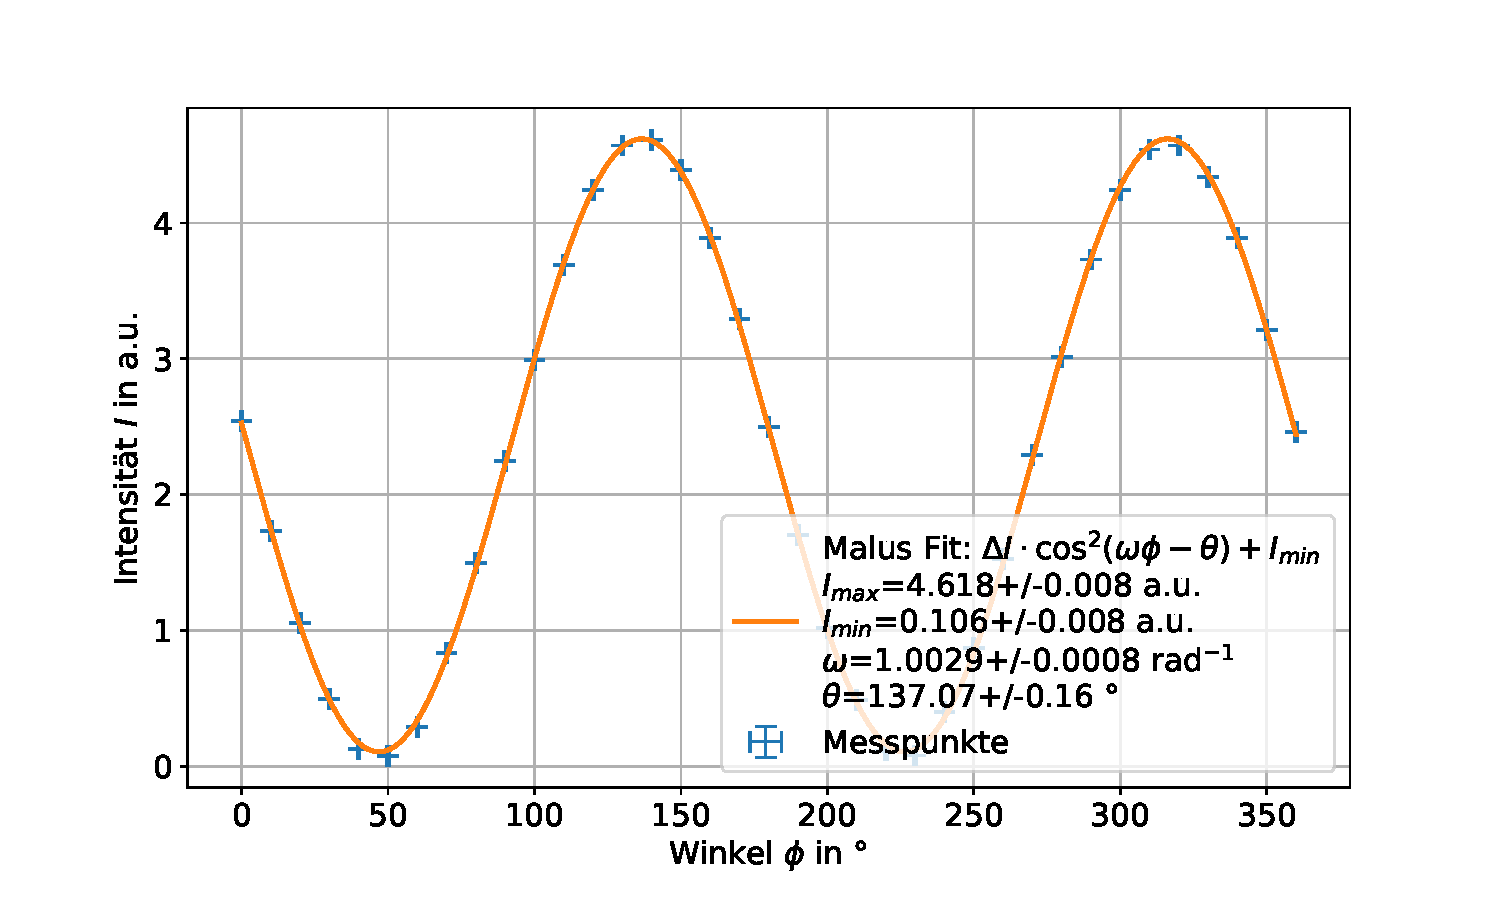
\includegraphics[width=0.8\linewidth]{img/malus}
			\caption{
			Messung der Intensität in Abhängigkeit vom Winkel des Polarisators.
			Die gelbe Funktion ist ein Fit nach dem Gesetzt von Malus.
			}
			\label{fig_malus}
	\end{figure}




			\subsubsection*{Diskussion}

			Wie in \cref{fig_malus} zu erkennen ist, spiegeln die Messpunkte sehr gut die nach dem Gesetz von Malus erwarte $\cos ^2$-Funktion wieder.
			In den Fitparametern ist außerdem festzustellen, dass in Frequenz $\omega$ zwar nicht innerhalb der Messunsicherheiten, aber doch sehr nahe an \num{1} liegt, was ebenfalls dem Gesetz von Malus entspricht (\cref{eq_malus}).
			\begin{equation}
				I = I_0 \cos^2(\alpha)
				\label{eq_malus}
			\end{equation}

			Dass im Gegensatz zu obiger Gleichung eine Phase auftritt, liegt darin, dass das Licht aus dem Laser in einem Winkel von \SI{137,07\pm 0.16}{\degree} zu einem Analysatorwinkel von Null gedreht linear polarisiert austritt.



		\subsection{Einstellung der Eingangspolarisation}
		%4.1.2
		% Kontrast für die vier Analysatorwinkel aus den Bildern (da steht explizit qualitativ. Reicht also wohl die Bilder zu printen und zu sagen: "Sieht man ja, wa?")
		% Intensitätsmessung 0 und 255 für horizontally divided
		In \cref{fig_divscreen} sind für vier Analysatorwinkel im Abstand von \SI{45}{\degree} die Kamerabilder aufgeführt.
		Hierbei wurde auf den LC-Modulator ein \textit{Horizontally Divided Screen} gegeben.
		\begin{figure}[H]
        \centering
        \begin{subfigure}[b]{0.475\textwidth}
            \centering
            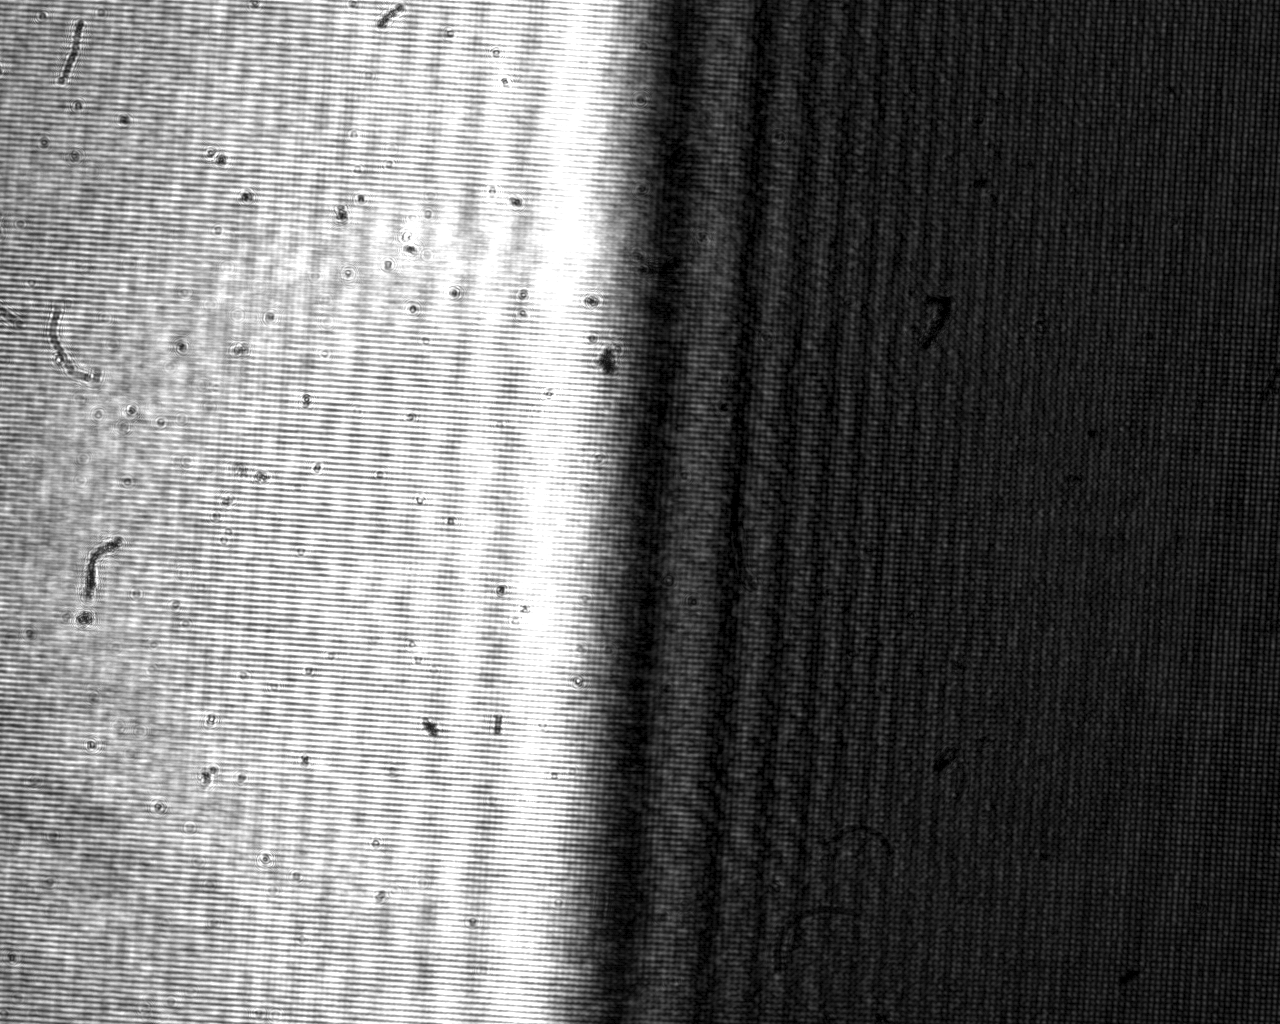
\includegraphics[width=\textwidth]{raw/dividedscreen_0_deg}
            \caption%
            {$\alpha=\SI{0}{\degree}$}
            \label{fig_divscreen_0}
        \end{subfigure}
        \hfill
        \begin{subfigure}[b]{0.475\textwidth}
            \centering
            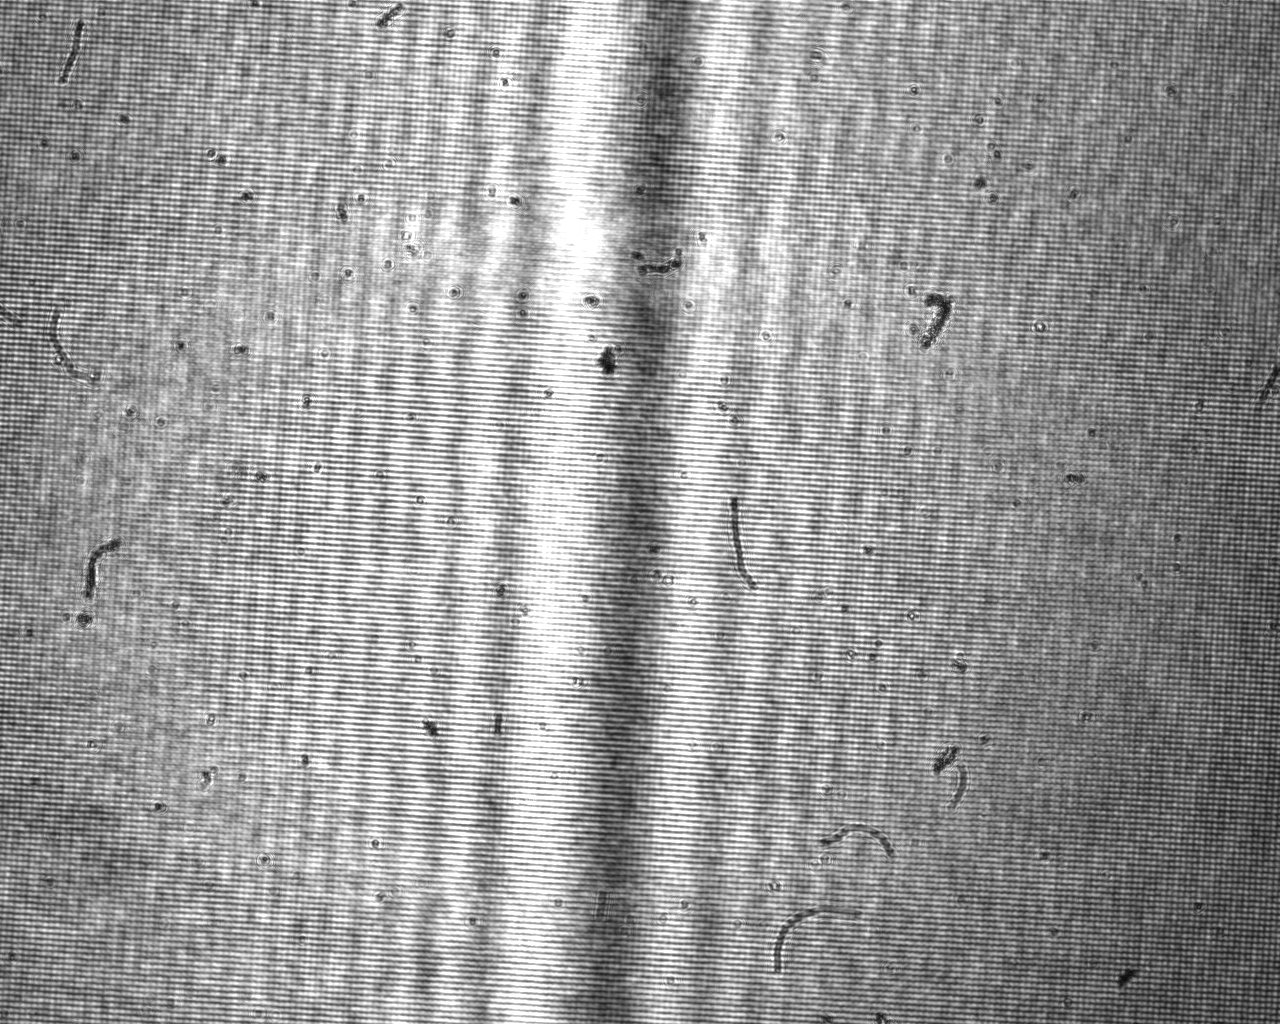
\includegraphics[width=\textwidth]{raw/dividedscreen_45_deg}
            \caption[]%
            {$\alpha=\SI{45}{\degree}$}
            \label{fig_divscreen_45}
        \end{subfigure}
        \vskip\baselineskip
        \begin{subfigure}[b]{0.475\textwidth}
            \centering
            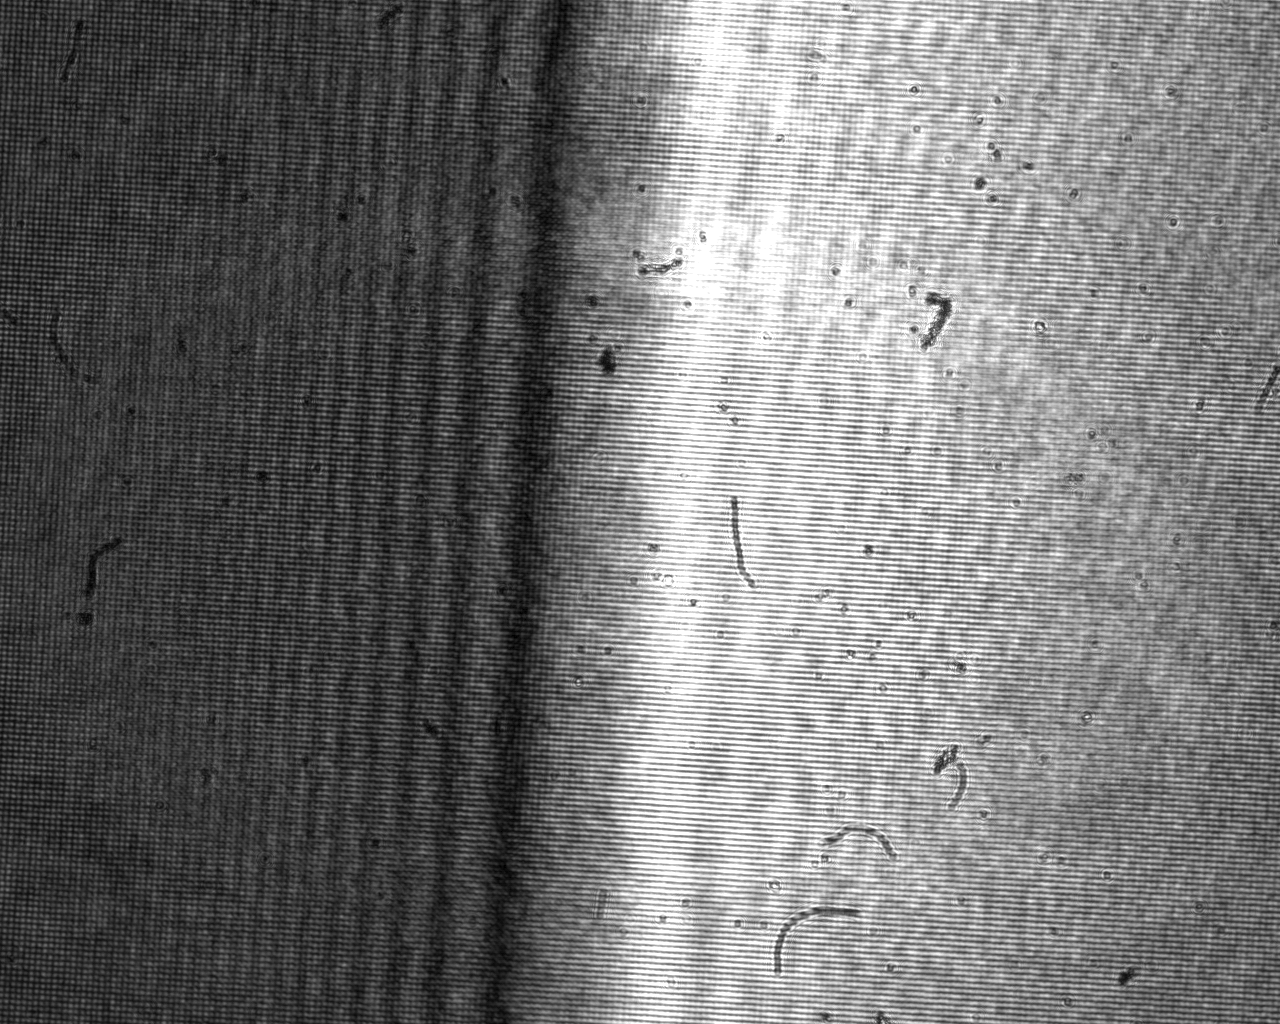
\includegraphics[width=\textwidth]{raw/dividedscreen_90_deg}
            \caption[]%
            {$\alpha=\SI{90}{\degree}$}
            \label{fig_divscreen_90}
        \end{subfigure}
        \quad
        \begin{subfigure}[b]{0.475\textwidth}
            \centering
            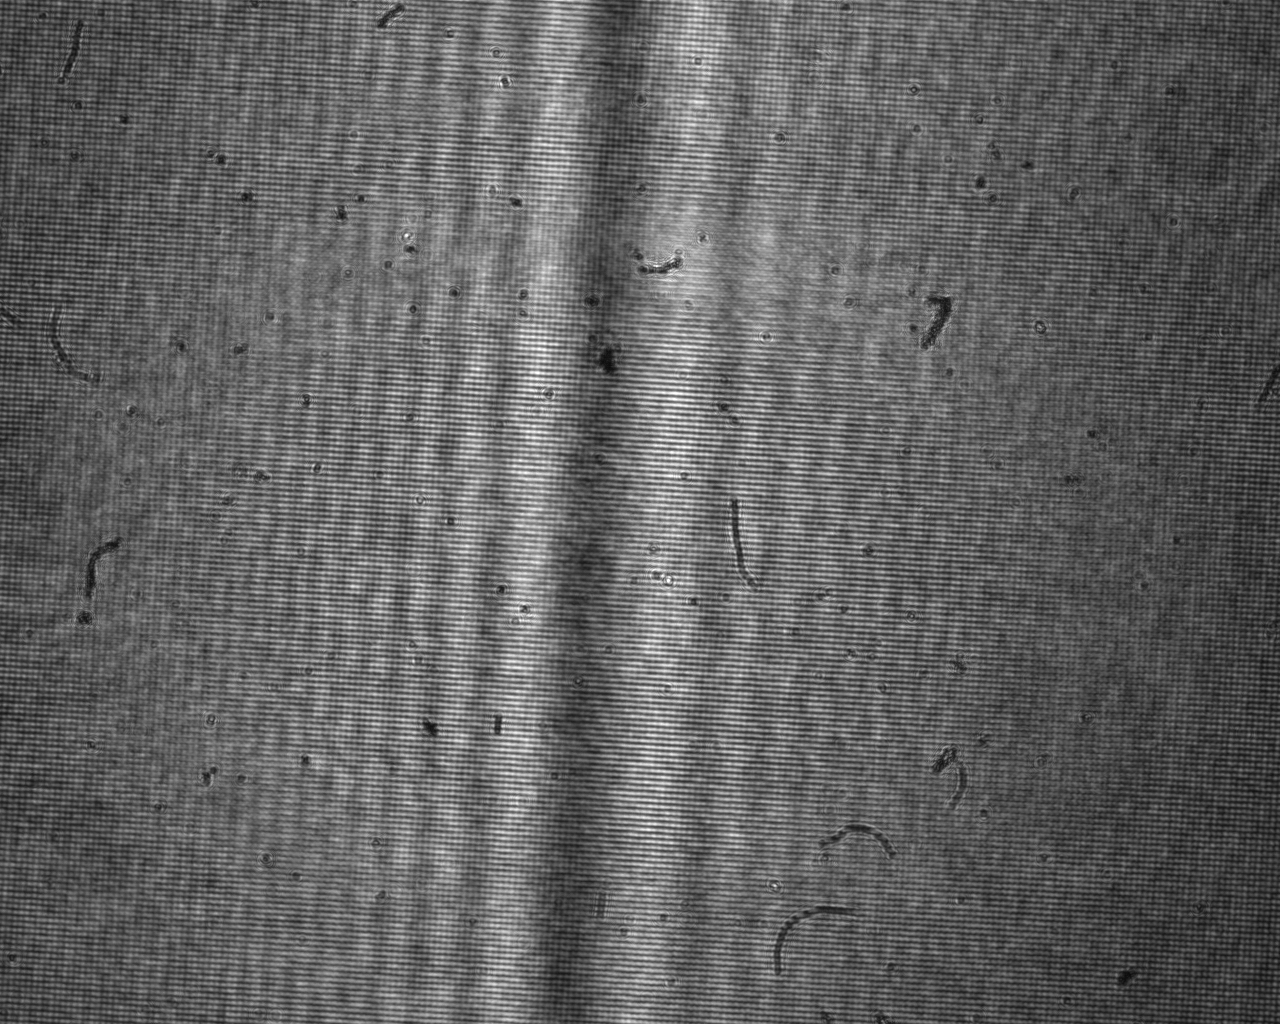
\includegraphics[width=\textwidth]{raw/dividedscreen_135_deg}
            \caption[]%
            {$\alpha=\SI{135}{\degree}$}
            \label{fig_divscreen_135}
        \end{subfigure}
        \caption%
        {Kameraaufnahmen für verschiedene Analysatorwinkel $\alpha$ mit einem \textit{Horizontally Divided Screen} auf dem LC-Modulator.}
        \label{fig_divscreen}
    \end{figure}


		Die Bestimmung des Kontrast erfolgt analog zu \cref{eq_kontrast} in \cref{ss_malus}, jedoch mit  den gemessenen Intensitäten $I_\text{max}=\input{res/intens_max}$ und $I_\text{min}=\input{res/intens_min}$, respektive für einen weißen und schwarzen \textit{Blank Screen}, sodass sich ein Kontrast von $C=\input{res/intens_kontrast}$ ergibt.
			\subsubsection*{Diskussion}
			% qualitativ: ist tatsächlich deutlich anders
			% Optimierung des Kontrastes bei LC-Modulator als Amplitudenmodulator beschreiben und erklären
			Zunächst lässt sich mittels \cref{fig_divscreen} die qualitativ die Erwartung bestätigen, dass bei der gewählten Eingangspolarisation von \SI{-135}{\degree}.
			Der Kontrast zwischen den beiden Flächen ist deutlich größer bei einem Analysatorwinkel von \SI{0}{\degree} bzw. \SI{90}{\degree} als für die dazu um \SI{45}{\degree} gekippten Polarisatorstellungen.
			Die Tatsache, dass $I_\text{min} = \input{res/intens_min}$ sich deutlich von Null unterscheidet zeigt, dass der LC-Modulator deutlich schlechter linear polarisiertes Licht ausgibt, als der Laser.
			Der berechnete Kontrast ist geringer als Herstellerangabe für den maximalen Kontrast von \SI{0,99}{} (vgl.\cite{Handbuch}).
			Dies kann an Verschmutzungen oder nicht vollständig optimierter Eingangspolarisation liegen.

			Dass das Bild auf der Kamera überhaupt wieder auftritt, liegt daran, dass am LC-Modulator eine Fouriertransformation stattfindet, die durch die Linse wieder rückgängig gemacht wird.
			Zusätzlich ist zu erkennen, dass sich ein Wellenmuster parallel zur Teilung des Bildschirms ergibt.
			Dies ist darauf zurückzuführen, dass die Rücktransformation unvollständig ist, da nur der Teil rücktransformiert wird, der auf die Linse trifft.
			Außerdem treten bei hohen Abständen zu optischen Achse oder großen Strahlenwinkeln zu optischen Achse Linsenfehler (sphärische Aberration und Astigmatismus) auf.
			Zusätzlich fallen kreisförmige Wellenmuster auf.
			Diese sind vermutlich Fouriertransformationen von punktförmigem Staub auf der Linse oder dem LC-Modulator.
			Nicht-fouriertransformierter Dreck auf der Kamera ist ebenfalls zu sehen.
			Theoretisch könnte der Dreck auch von der Laserlinse stammen und hin- und rücktransformiert sein, aber dann wären die gleichen Wellenstrukturen, wie beim \textit{Horizontally Divided Screen} zu erwarten.

			Dass ein eingangspolarisationsabhängiger Kontrast auftritt, liegt an der Rotation der Lichtpolarisation durch die Helixstruktur in den LC-Zellen.
			Wenn das Licht parallel zum Polarisationsfilter am Eingang der LC-Zelle ankommt, wird es zu einem hohen Anteil transmittiert, wenn keine Spannung anliegt und zu einem geringen transmittiert wenn Spannung anliegt.
			Der Kontrast ist also hoch.

		\subsection{Bestimmung der Pixelgröße} %: Achtung, ich habe hier die beiden zusammengechoben und den dazwischen dahinter geschoben
		%TODO Konsistenz mit Pixelabstand vs Pixelgröße
		Die verwendete Linse hat eine Brennweite $f$ von \SI{20+-0.3}{cm} und die Wellenlänge $\lambda$ des HeNe-Lasers beträgt \SI{632.8}{nm}.
			\subsubsection*{Variante 1}
			%4.1.3
			% ausrechnen und Messungenauigkeit abschätzen

			Die Größe $G$ des \SI{200}{}x\SI{200}{} Pixel Quadrats auf dem LC-Display lässt sich aus Bildgröße $B$, Bildweite $b$ und Brennweite $f$ mit \cref{eq_fokus} berechnen. %TODO x mathmode?
			Der Pixelabstand $p$ ergibt sich aus dem Quotienten von $G$ und Höhe des Quadrats in Pixeln.
			Für die Unsicherheit $u$ der Höhe des Quadrats in Pixeln wird einen Rechteckverteilung  von $u = \frac{\SI{10}{px}}{2\sqrt{3}}= \SI{3}{px}$ verwendet, da Bilder von 800x600 Pixel auf den LC-Modulator mit 824x624 Pixel skaliert werden und auch der Rahmen des Bildprogramms mit an den LC-Modulator übertragen wird.
			Die Messungen sowie der resultierende Pixelabstand $p$ sind in \cref{tb_pixel} tabelliert.
			\begin{equation}
				\label{eq_fokus}
				G = \frac{B}{b/f-1}
			\end{equation}

\begin{table}[H]
		\centering
		\begin{tabular}{ c | c | c | c }
			 Bildweite $b/\si{cm}$ & Bildgröße $B/\si{cm}$ & Größe $G/\si{cm}$ & Pixelabstand $p/\si{\mu m}$ \\ \hline
			 \input{res/tb_pixel}
		\end{tabular}
		\caption{
		Gemessene Bildweite $b$, Bildgröße $B$ und berechnete Größe $G$, Pixelgröße $p$.
		}
		\label{tb_pixel}
\end{table}
			\subsubsection*{Variante 2}
			%4.2.1
			% ausrechnen

			Für Beugung an einem Gitter mit der Gitterkonstanten $g$ gilt für das $m$. Maximum:
			\begin{equation}
				g \cdot \sin{\alpha} = m \lambda
			\end{equation}
			Für kleines $\alpha$ gilt $\alpha\approx\sin{\alpha}\approx\tan{\alpha}=\frac{d}{2f}$, wobei $d$ der Abstand zwei Maxima gleicher Ordnung $m$  zueinander ist und somit:
			\begin{equation}
				g = \frac{2m\lambda f}{d}
			\end{equation}



\begin{table}[H]
		\centering
		\begin{tabular}{ c | c | c }
			 Ordnung $m$ & Abstand $d/\si{cm}$ & Pixelabstand $p/\si{\mu m}$ \\ \hline
			 \input{res/tb_gitter}
		\end{tabular}
		\caption{
		Gemessener Abstand $d$, Bildgröße $B$ und berechnete Pixelgröße $p$.
		}
		\label{tb_gitter}
\end{table}
			\subsubsection*{Diskussion}
			% beide Werte mit Materialbeschreibung vergleichen. aus der Anleitung von dem SLM?
			Wenn man die gemessenen Pixelabstände in \cref{tb_pixel} und \cref{tb_gitter} mit der Herstellerangabe gemäß \cite{Handbuch} von \SI{32}{\micro \meter}, die auf \SI{\pm 3}{\micro \meter} genau bestimmt werden können soll, vergleicht, stellt man fest, dass dies innerhalb der Messunsicherheiten der Fall ist. % geiler Satz.


		\subsection{Zusammenhang zwischen Grauwert und Polarisationszustand}
		%4.1.4
		% plotten
		In \cref{fig_ellipse} ist die Exzentrizität des Lichts in Polarkoordinaten dargestellt.
		Die maximal gemessene Intensität $I_\text{max}$ unter Variation des Analysatorwinkels bei einem \textit{Blank Screen} mit einem gewissen Grauwert wird als Länge der großen Halbachse einer Ellipse aufgefasst.
		Die kleine Halbachse ergibt sich aus der minimalen Intensität $I_\text{min}$, also unter einer Analysatorwinkeländerung von \SI{90}{\degree}.
		Zusätzlich wird die Hauptachse der Ellipse um den Analysatorwinkel gegenüber der x-Achse rotiert.


\begin{figure}[H]
			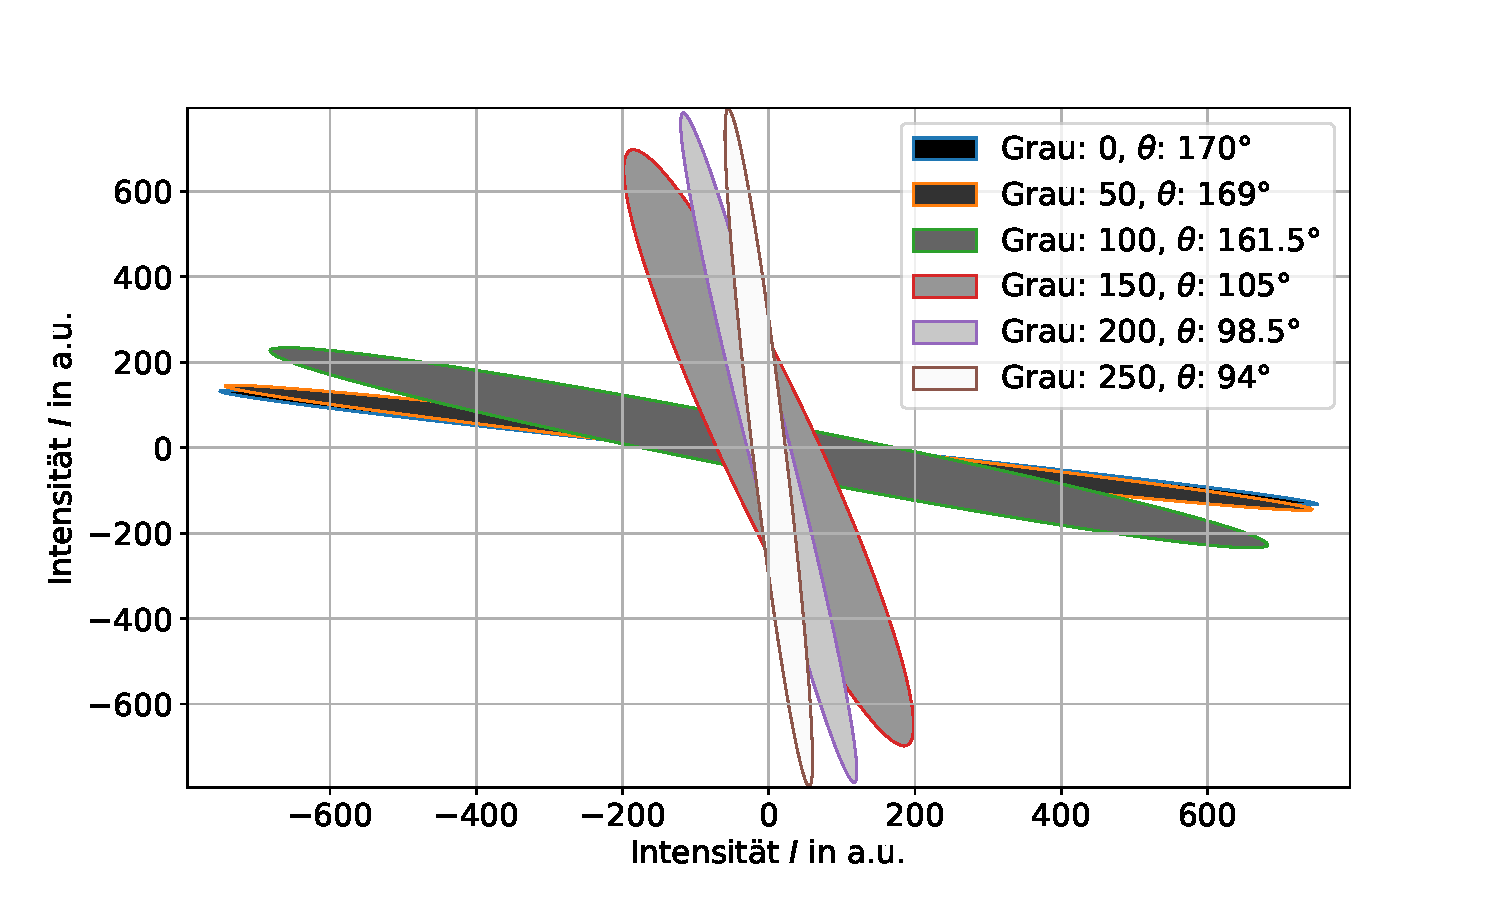
\includegraphics[width=1\linewidth]{img/ellipse}
			\caption{
			Exzentrizität des Lichts.
			Die maximale Intensität $I_\text{max}$ entspricht der großen Halbachse, welche um den Analysatorwinkel $\theta$ zur x-Achse rotiert ist.
			Die kleine Halbachse ist die Intensität $I_\text{min}$.
			Die Daten stammen aus \cite{JTZ}.
			}
			\label{fig_ellipse}
	\end{figure}

			\subsubsection*{Diskussion}
			% Zusammenhang zwischen Grauwert und Drehwinkel erklären. Wie ist die Ausrichtung der Flüssigkristalle im LC-Modulator ohne Angelegte Spannung-> helix obv.
			Die Polarisation dreht sich mit dem Grauwert und die Exzentrizität wird bei einem mittleren Grauwert minimal.
			Ersteres liegt daran, dass bei einem \textit{Blanc Screen} der gesamte LC-Modulator näherungsweise als eine LC-Zelle aufgefasst werden kann.
			Diese dreht ohne angelegte Spannung die Polarisation des Lichtes um \SI{90}{\degree}.
			Bei maximaler Spannung dreht sie die Polarisation nicht mehr.
			Da der eingestellte Grauwert invers der angelegten Spannung entspricht (hoher Grauwert bedeutet hohe Durchlässigkeit der Zellen), wird hierdurch die Grauwertabhängigkeit der Ausgangspolarisation erklärt.
			Eine geringe Exzentrizität entspricht einer starken durchschnittlichen Abweichung von der Vorzugspolarisationsrichtung.
			Hier ist das Licht also weniger einheitlich polarisiert.
			Dass dies bei einem mittleren Grauwert der Fall ist, zeigt, dass bei mittlerer angelegter Spannung nicht bei allen LC-Zellen die Polarisation gleich weit gedreht wird, während dies bei komplett fehlender oder maximaler Spannung eher der Fall ist.

		\subsection{Intensitätsverteilung in den Beugungsordnungen des unadressierten Displays}
		%4.2.2
		% Trennung horzontale und vertikale Strukturen
		% Intensität bei 1-10 plotten
		% duty cycle bestimmen: Verhältnis transparenter Teil / lichtundurchlässiger Teil anhand der Intensitätsmodulation
		% Füllfaktor (Verhältnis transparent / gesamt) abschätzen: pixel quadratisch. -> ??? Dann ergibt sich der Füllfaktor doch instant aus dem duty cycle. Das klingt aber sehr anders gemeint in 4.2.2
		% hast du hier jetzt einfach auch die Werte von Jannik genommen? Steht nirgendwo und ist halt bissl meh, weil wir haben ja Werte, nur halt horizontal nicht so viele.

		Der Tastgrad $c$ ist definiert als das Verhältnis einer Impulsdauer $\tau$ zur Periodendauer $T$, also $c=\tau/T$.
		Übertragen auf die Transparenz der Pixel ist $c=t/g=1-i/g$.
		Wobei $t$ die Ausdehnung des transparenten, $i$ des intransparenten und $g=i+t$ des gesamten Pixels beschreibt.


		Für Gitter gilt, dass das Produkt aus Periodizität im Realraum $r$ und reziproken Raum $P$ konstant ist, $rP=\text{const.}$.
		Im Experiment sind zwei Gitter simultan vorhanden, welche beide eine Fouriertransformation zur Folge haben.
		Ein Gitter definiert die Pixelgröße und eines entstammt der Steuerelektronik, die als ebenfalls periodisch, also als für jeden Pixel gleich aussehend, angenommen wird.
		Somit kann angenommen werden, dass:
		\begin{equation}
			gG = iI = \text{const.}
		\end{equation}
		Wobei $G$ und $I$ die respektiven Periodizitäten im reziproken Raum sind und es folgt, dass sich das Transparenzverhältnis $c=1-i/g=1-G/I$ im reziproken Raum als Verhältnis der Frequenzen widerspiegelt.

		In \cref{fig_sinc1} sind die Intensitäten der vertikalen Maxima aufgetragen.
		Maxima sind deutlich bei $m=\{0,4,7,9\}$ und Minima bei $m=\{3,6,8\}$.
		Der geringe Abstand zwischen den Maxima $\{7,9\}$ und dem Minimum $\{8\}$, lässt darauf folgern, dass im Bereich nahe der 0. Ordnung ein weiteres Minimum existiert, aber nicht aufgelöst werden konnte.
		Und es lässt sich das Verhältnis der Frequenzen durch das Verhältnis der Maxima beschreiben $c_v=1-4/9$.
		Da in \cref{fig_sinc2} lediglich die ersten 6 Maxima aufgelöst werden konnten ist eine weitere Auswertung damit nicht möglich, jedoch mit \cref{fig_sinc3}, welche sich in dem Bereich von 0. bis 6. Maximum sehr ähnlich verhält.
		Somit stellt man analog in \cref{fig_sinc3} fest, dass $c_h=1-2/9$ beträgt und ebenfalls das erste Minimum nicht aufgelöst werden konnte.
		Mit einer Betrachtung der Unsicherheit, welche durch eine Rechteckverteilung der Breite 1 am Punkt $m=9$ abgeschätzt wird, folgen mit $m=\SI{9+-0.3}{}$ Tastgrade von $c_v=\SI{0.556(15)}{}$ und $c_h=\SI{0.778(7)}{}$.
		Die Rechteckverteilung wird angenommen, da wenn das Maximum sich irgendwo zwischen \num{8,5} oder \num{9,5} befindet, es dazu führt, dass man es beim Punkt \num{9} sieht, da zwischen den Maxima des Pixelgitters nicht gemessen werden kann.

		Als grobe Abschätzung ergibt sich der Füllfaktor aus dem Produkt der Tastgrade:
		\begin{equation}
			\text{FF} \approx c_v c_h =\SI{43.2+-1.2}{\percent}
		\end{equation}


\begin{figure}[H]
			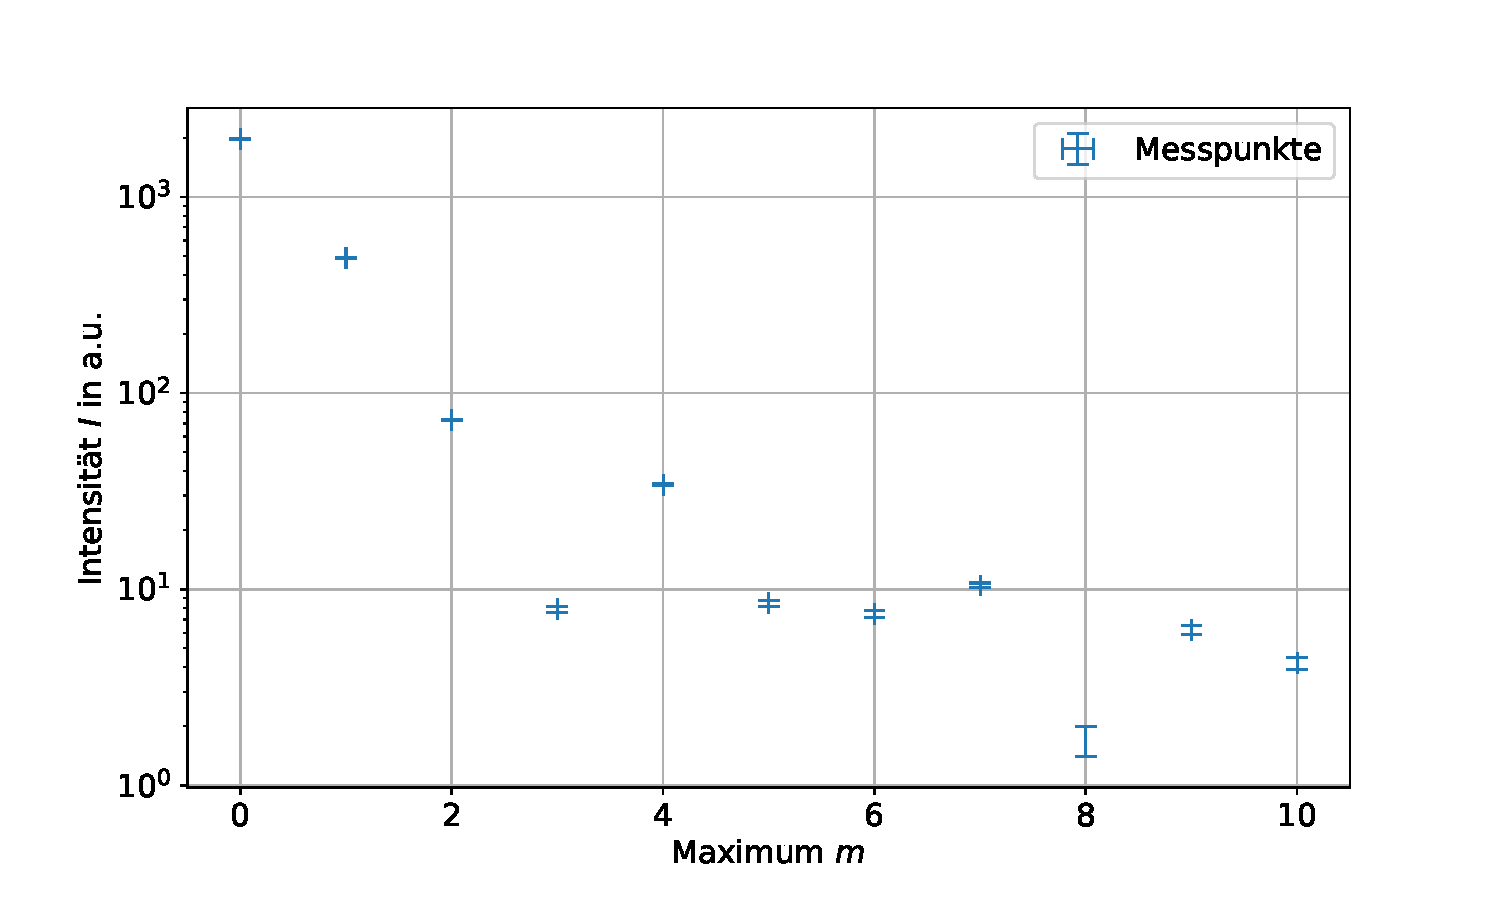
\includegraphics[width=0.8\linewidth]{img/sinc1}
			\caption{
			Messung der Intensität in Maxima der Gitterbeugung (durch das Pixelgitter) in vertikaler Richtung.
			}
			\label{fig_sinc1}
	\end{figure}

\begin{figure}[H]
			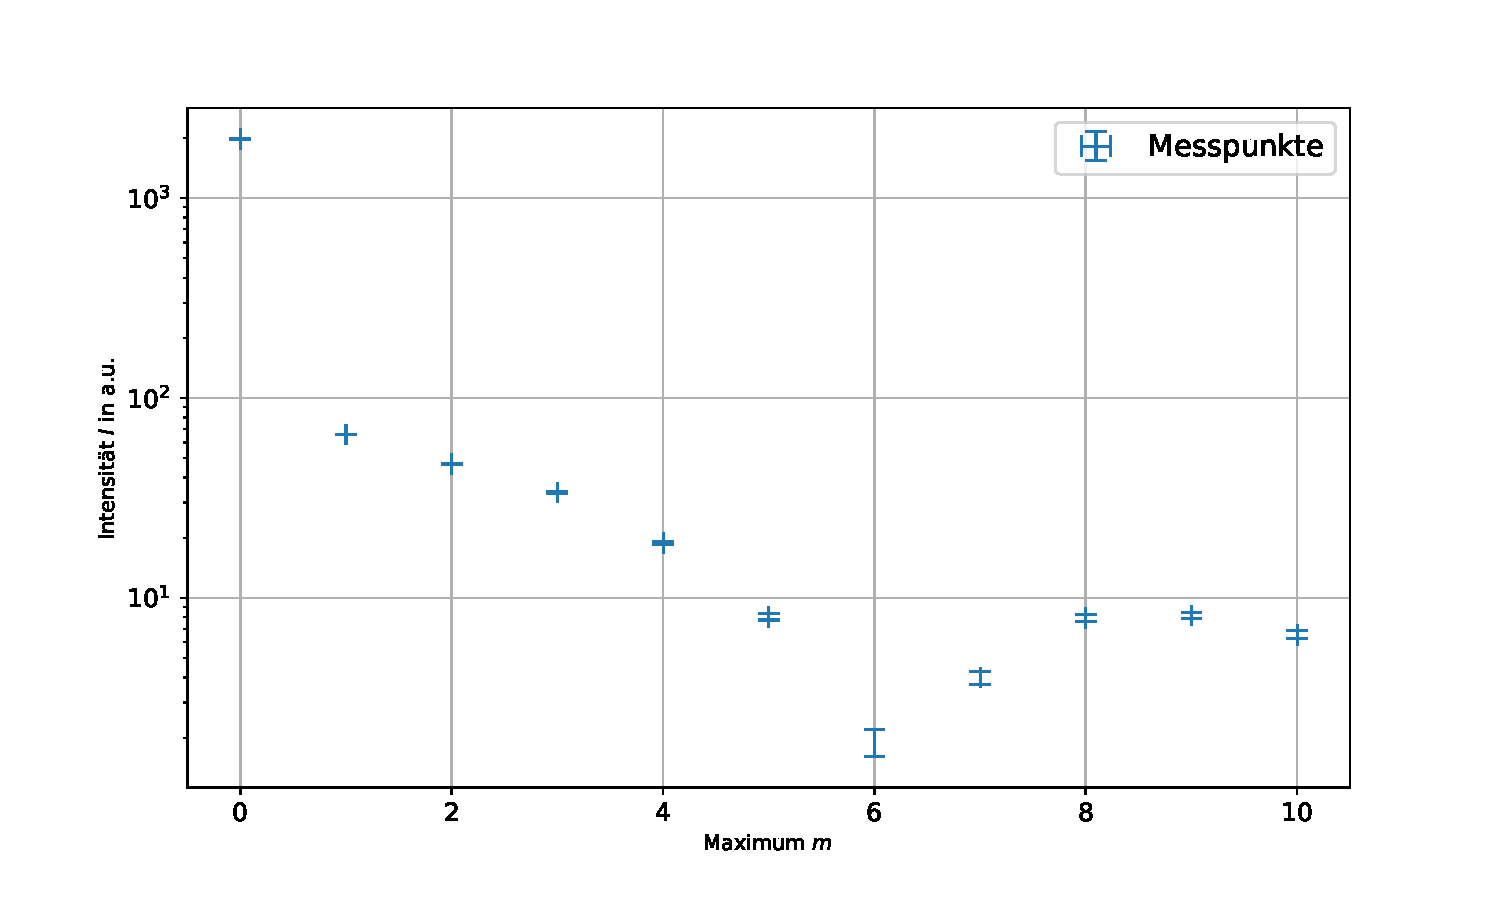
\includegraphics[width=0.8\linewidth]{img/sinc2}
			\caption{
			Messung der Intensität in Maxima der Gitterbeugung (durch das Pixelgitter) in horizontaler Richtung.
			}
			\label{fig_sinc2}
	\end{figure}

\begin{figure}[H]
			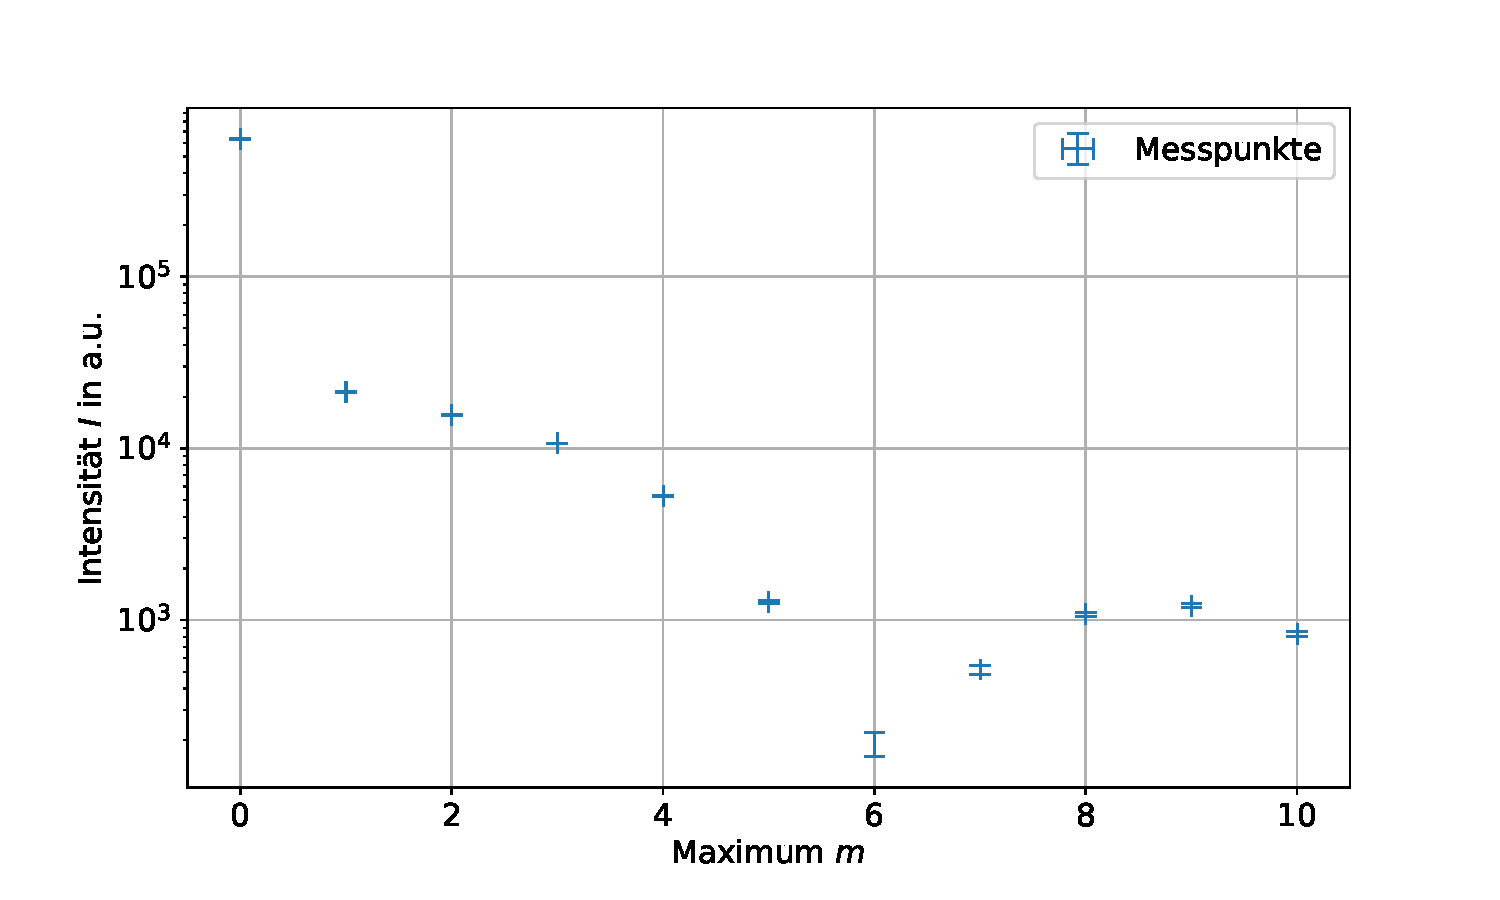
\includegraphics[width=0.8\linewidth]{img/sinc3}
			\caption{
			Messung der Intensität in Maxima der Gitterbeugung (durch das Pixelgitter) in horizontaler Richtung.
			Die Daten stammen aus \cite{JTZ}.
			}
			\label{fig_sinc3}
	\end{figure}


			\subsubsection*{Diskussion}
			% Warum Untermodulation?
			Horizontale Strukturen sind durch ihre Höhe definiert und vertikale durch ihre Breite.
			Außerdem verursacht ein Gitter mit vertikalen Spalten ein horizontales Beugungsbild und umgekehrt.
			Dementsprechend entspricht der vertikale Tastgrad horizontalen Strukturen und umgekehrt.

			Der abgeschätzte Füllfaktor von \SI{43,2\pm 1,2}{\percent} ist um mehr als die Messunsicherheit geringer als der in \cite{Handbuch} angegebene von etwa \SI{55}{\percent}.

			Jedoch ist die Messung durch die Ordnungen des Pixelgitters eingeschränkt:
			Wenn man die Untermodulation durch elektrische Ansteuerungselemente als periodisches Signal mit einer räumlichen Frequenz $ f_\text{Signal} $ in vertikaler oder horizontaler Richtung auffasst und die Messabstände durch das Pixelgitter als eine räumliche Abtastrate $f_\text{Abtast}$ interpretiert, muss gemäß der Signaltheorie $f_\text{Abtast} > 2 f_\text{Signal}$ (vgl. Nyquistfrequenz).
			Ansonsten treten Aliasing-Effekte auf.
			Dies kann bei dem gegebenen Aufbau allerdings nicht sichergestellt werden.

		\subsection{Beugungsbilder verschiedener DOEs}
		%4.2.3
		% Bilder
		% Beugungswirkungsgrad bestimmen
 		\cref{fig_doe_mix} zeigt jeweils 2 Beugungsbilder von einem Einzelspalt, Doppelspalt und Gitter.
		\begin{figure}[H]
        \centering
        \begin{subfigure}[b]{0.475\textwidth}
            \centering
            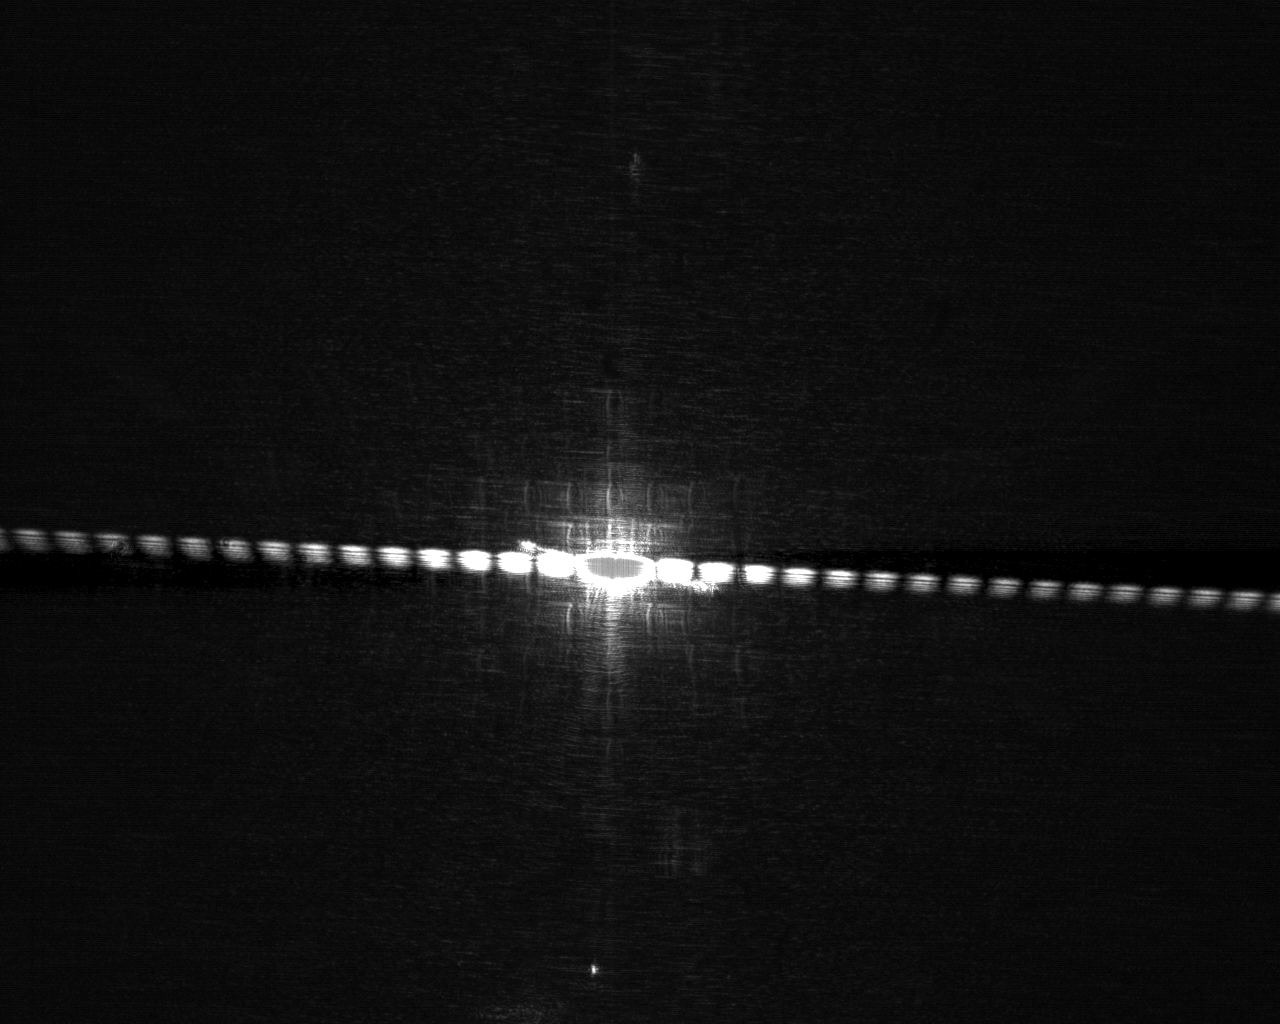
\includegraphics[width=\textwidth]{raw/singleslid_20_width}
            \caption%
            {Einzelspalt: Breite $\SI{20}{px}$}
            \label{fig_singleslid_20}
        \end{subfigure}
        \hfill
        \begin{subfigure}[b]{0.475\textwidth}
            \centering
            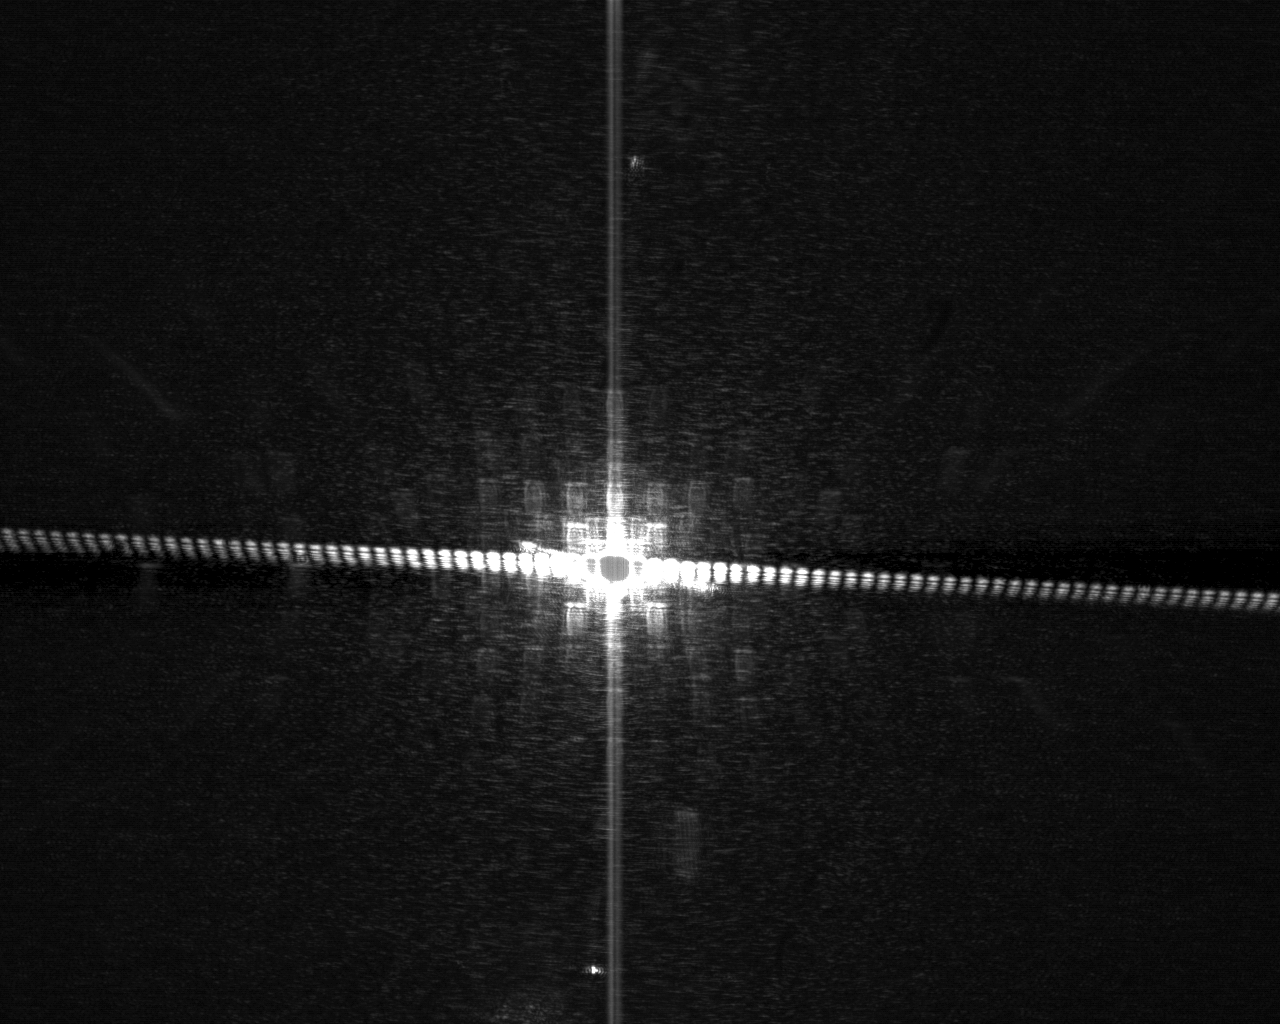
\includegraphics[width=\textwidth]{raw/singleslid_50_width}
            \caption%
            {Einzelspalt: Breite $\SI{50}{px}$}
            \label{fig_singleslid_50}
        \end{subfigure}
        \vskip\baselineskip
        \begin{subfigure}[b]{0.475\textwidth}
            \centering
            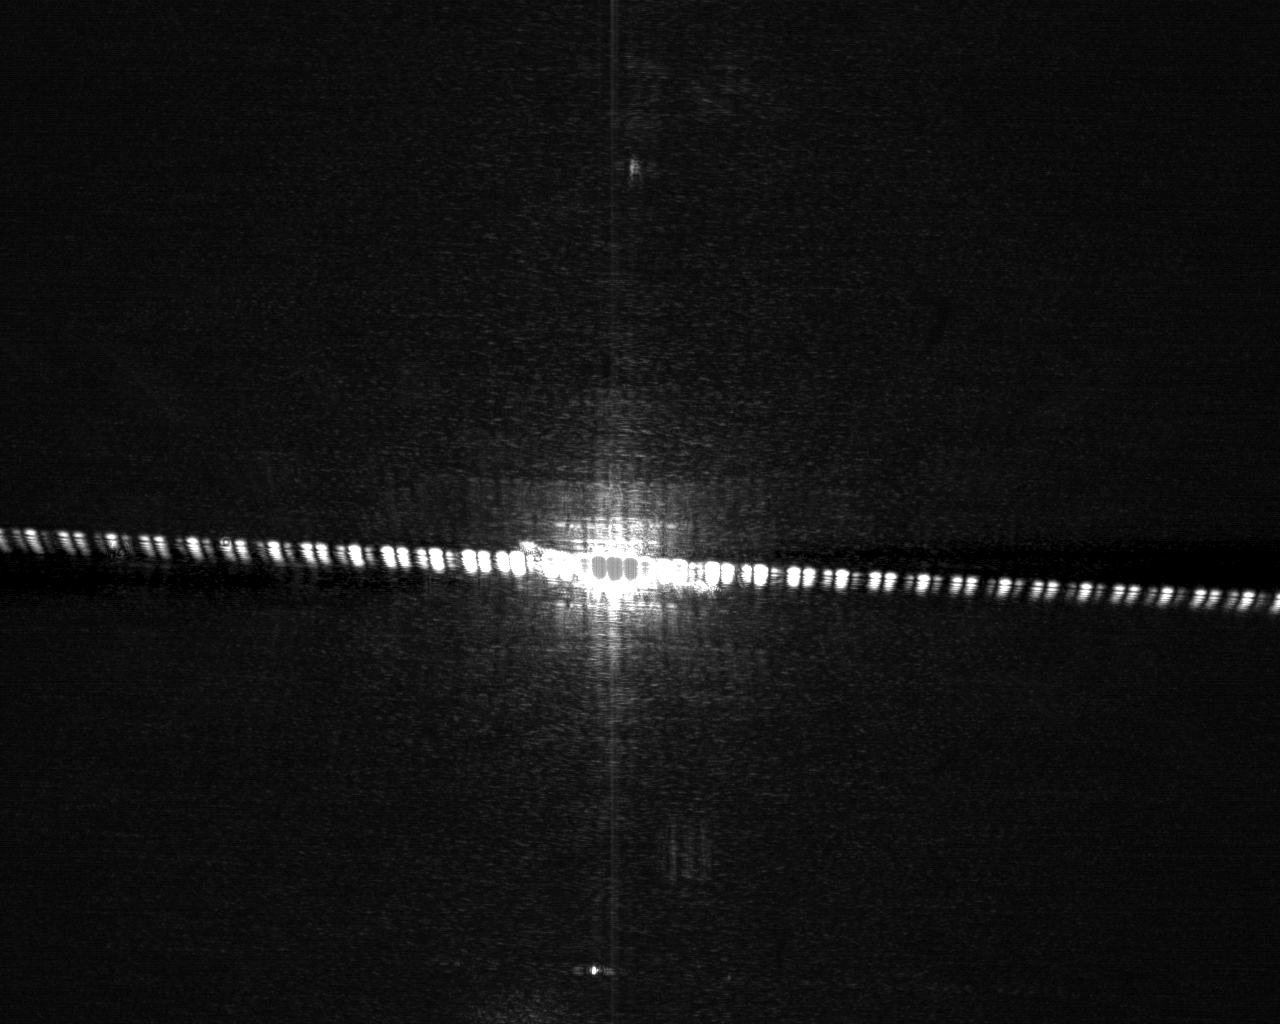
\includegraphics[width=\textwidth]{raw/doubleslit_20_width_50_dist}
            \caption[]%
            {Doppelspalt: Breite: \SI{20}{px}, Abstand: \SI{50}{px}}
            \label{fig_doubleslit_20_50}
        \end{subfigure}
        \quad
        \begin{subfigure}[b]{0.475\textwidth}
            \centering
            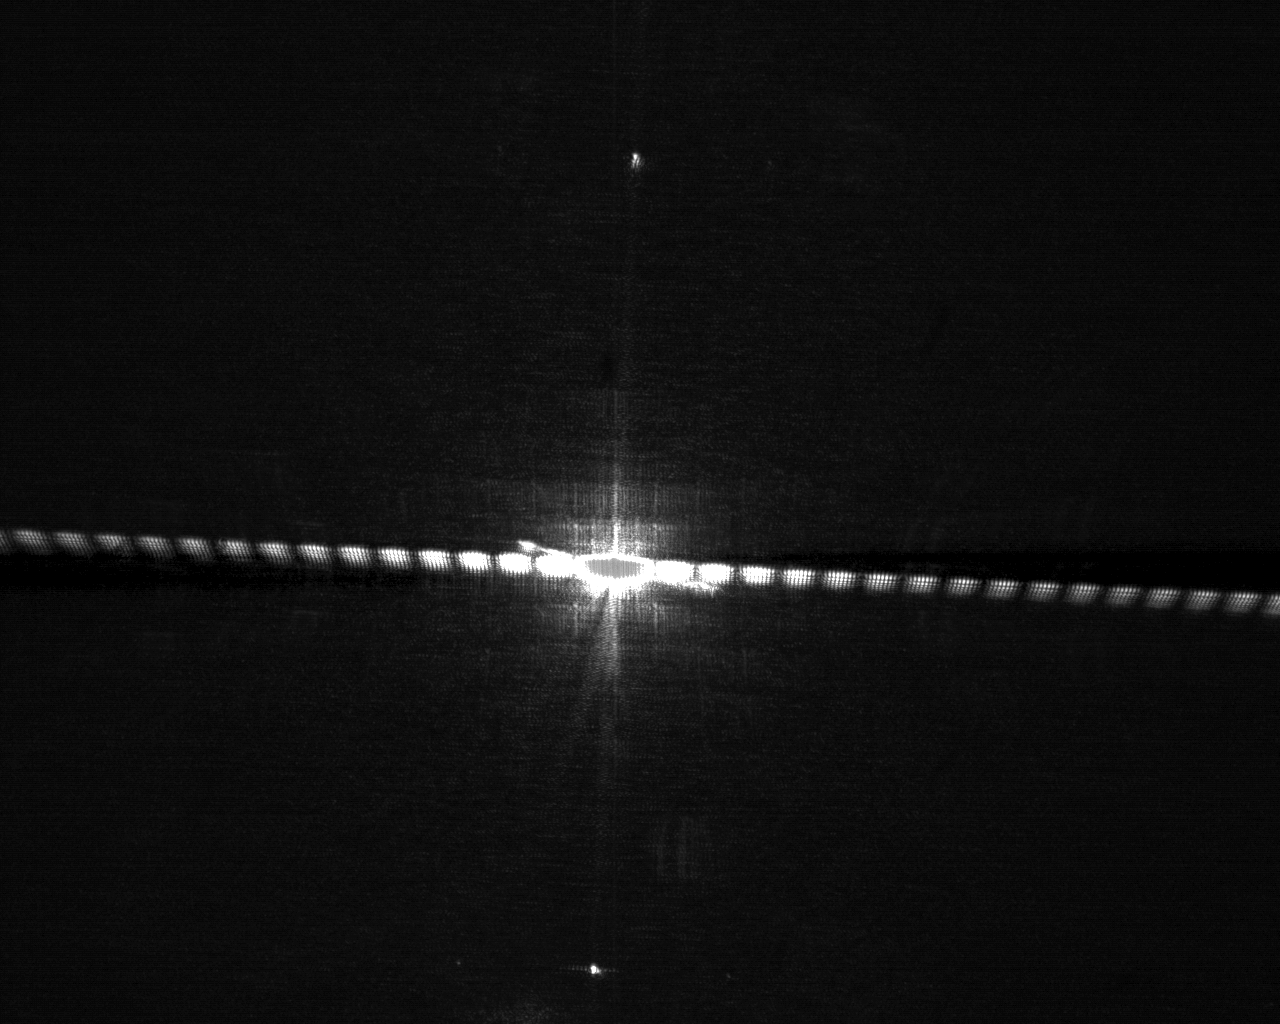
\includegraphics[width=\textwidth]{raw/doubleslit_20_width_200_dist}
            \caption[]%
            {Doppelspalt: Breite \SI{20}{px}, Abstand: \SI{200}{px}}
            \label{fig_doubleslit_20_200}
        \end{subfigure}
        \vskip\baselineskip
        \begin{subfigure}[b]{0.475\textwidth}
            \centering
            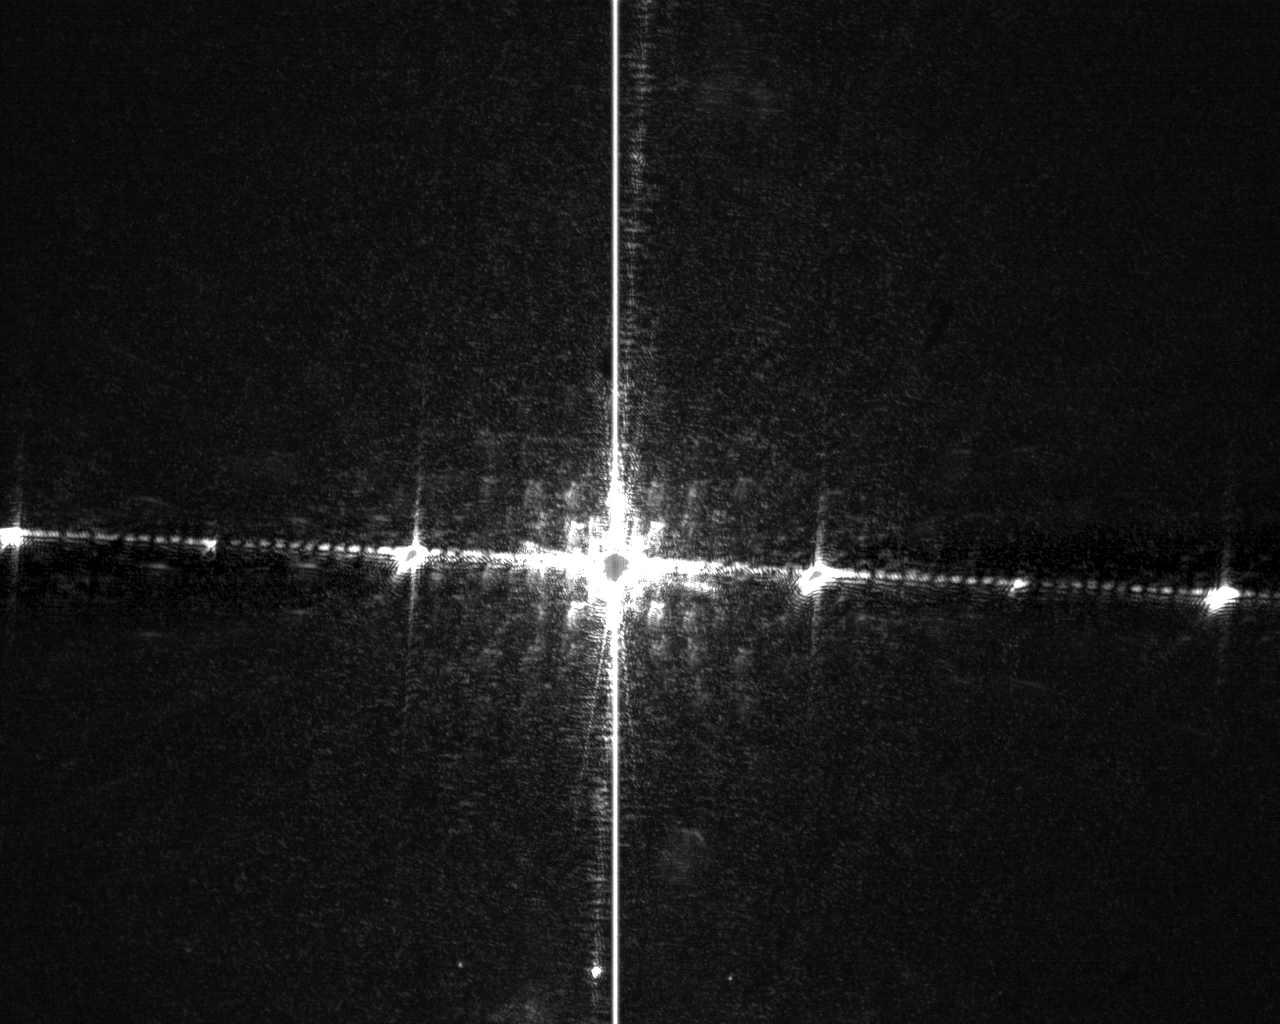
\includegraphics[width=\textwidth]{raw/grid_2_groove_2_ridge}
            \caption[]%
            {Gitter: Lücke: \SI{2}{px}, Steg: \SI{2}{px}}
            \label{fig_grid_2_2}
        \end{subfigure}
        \quad
        \begin{subfigure}[b]{0.475\textwidth}
            \centering
            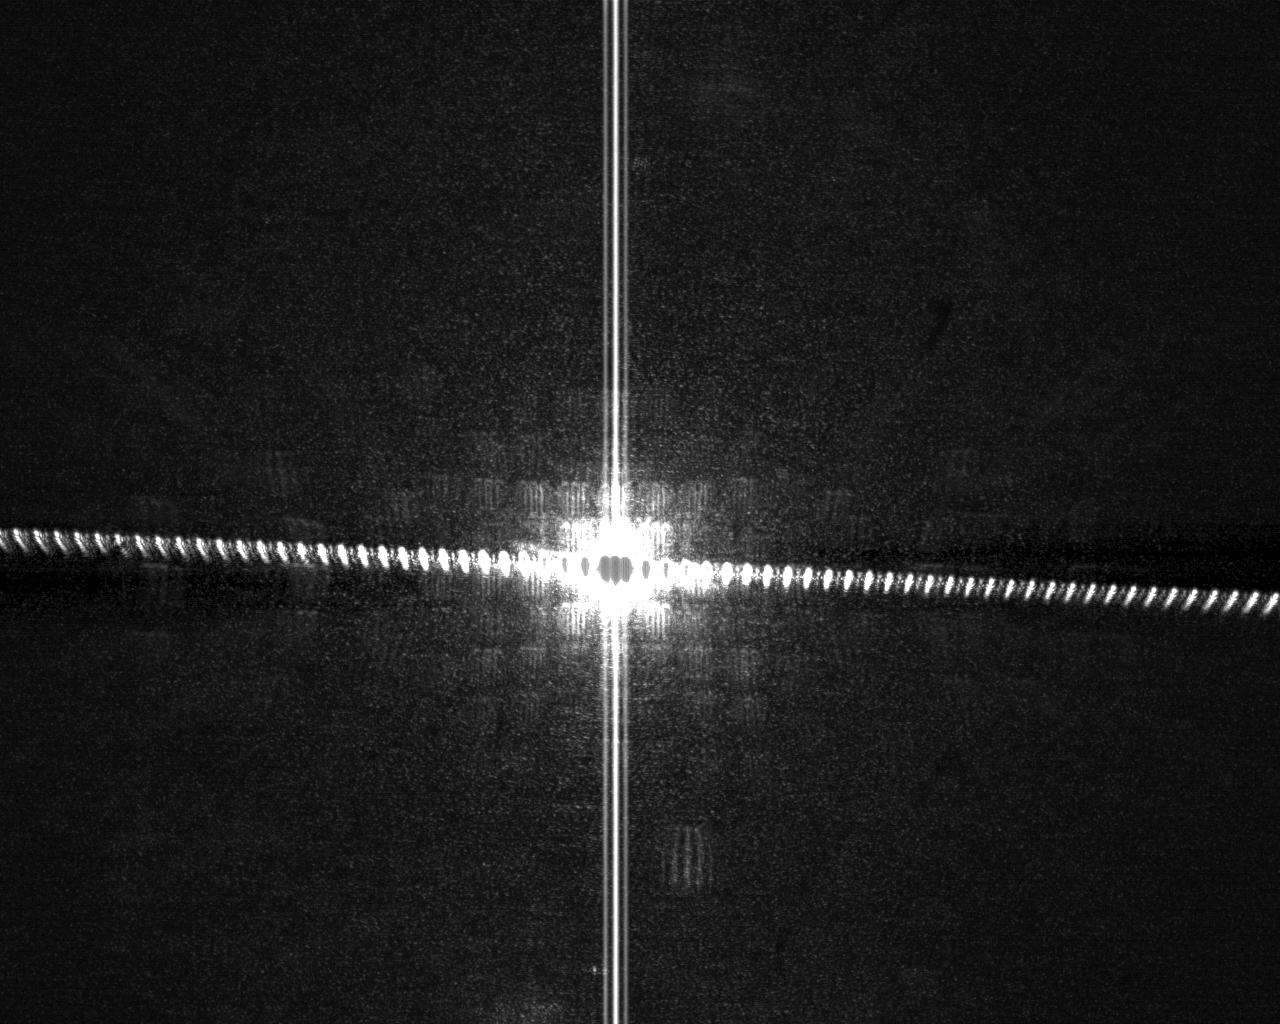
\includegraphics[width=\textwidth]{raw/grid_40_groove_40_ridge}
            \caption[]%
            {Gitter: Lücke: \SI{40}{px}, Steg: \SI{40}{px}}
            \label{fig_grid_40_40}
        \end{subfigure}
        \caption%
        {Kameraaufnahmen verschiedener Beugungsbilder}
        \label{fig_doe_mix}
    \end{figure}

		Über \cref{eq_beug} ist der Beugungswirkungsgrad $\eta$ definiert.
		\begin{equation}
			\label{eq_beug}
			\eta = \frac{I_\text{1,max}}{I_\text{0,max}}
		\end{equation}
		Es wurde ein Gitter mit Lücke und Steg von jeweils \SI{20}{px} verwendet.
		In \cref{tb_beug} und \cref{fig_beug} sind die Messwerte und resultierende Beugungswirkungsgrade angegeben.
\begin{table}[H]
		\centering
		\begin{tabular}{ c | c | c | c }
			 Grauwert & $I_\text{0,max}/$a.u. &$I_\text{1,max}/$a.u.&  Beugungswirkungsgrad $\eta$ \\ \hline
			 \input{res/tb_beug}
		\end{tabular}
		\caption{
		Gemessene Intensitäten der 0. und 1. Hauptmaxima eines Gitters bei verschiedenen Grauwerten.
		Der Beugungswirkungsgrad ergibt sich aus dem Quotienten der Intensitäten nach \cref{eq_beug}.
		}
		\label{tb_beug}
\end{table}
\begin{figure}[H]
			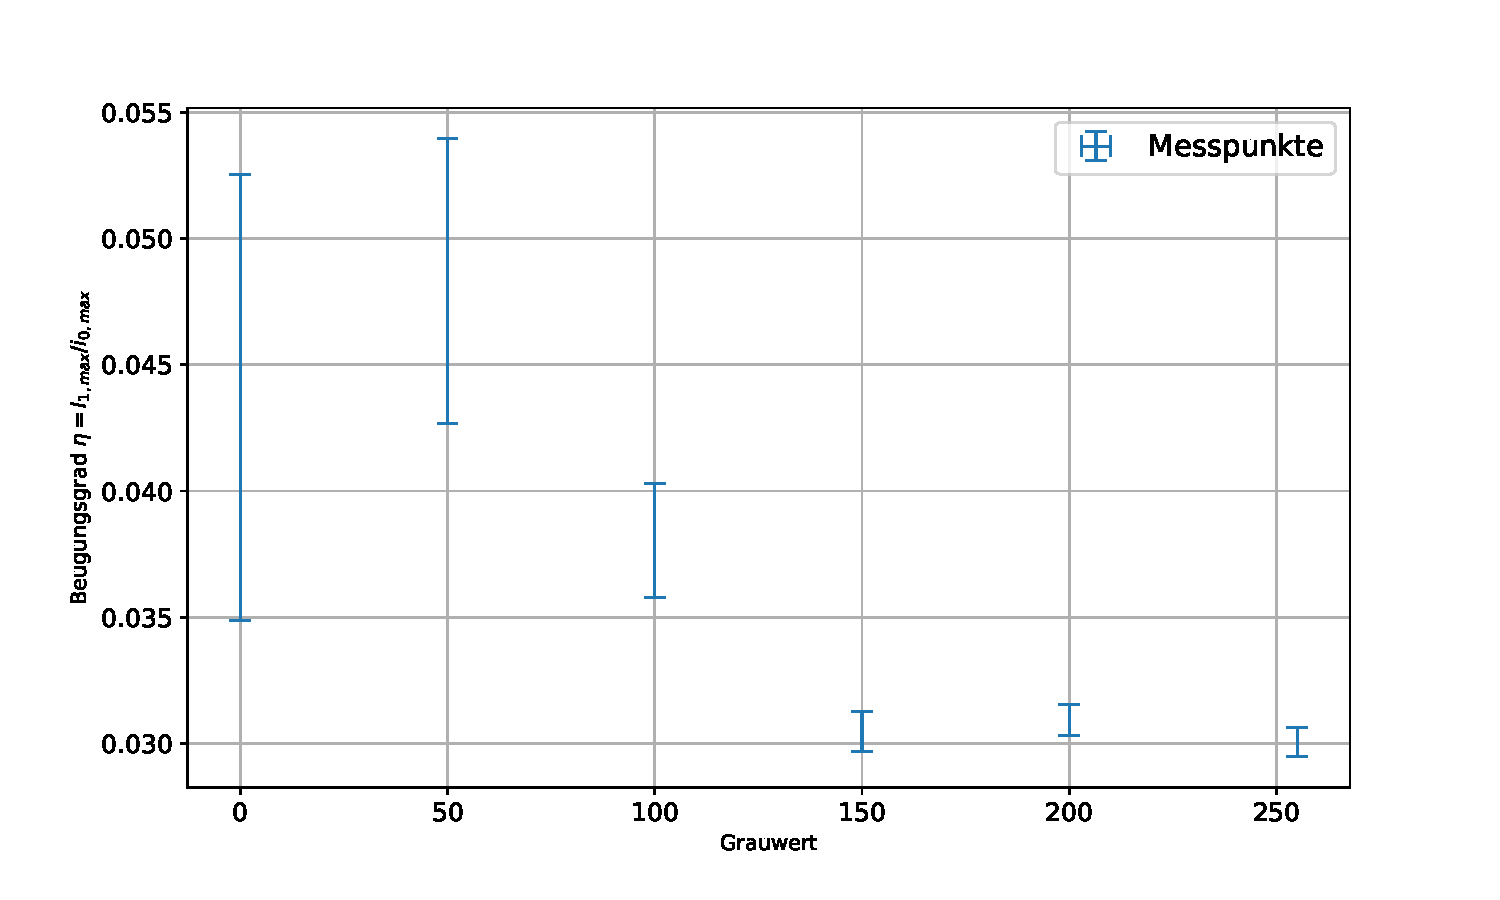
\includegraphics[width=0.8\linewidth]{img/beugungsgrad}
			\caption{
			Messung der Intensität in Maxima der Gitterbeugung in horizontaler Richtung.
			}
			\label{fig_beug}
	\end{figure}

			\subsubsection*{Diskussion}
		% Beobachtung, Änderung mit Strukturgröße
			% Warum kann ein LC-Modulator Beugungsbilder erzeugen?
			Die Intensität der Maxima nimmt, wie in \cref{tb_beug} zu erkennen ist, mit dem Grauwert zu.
			Dies entspricht der trivialen Erwartung, dass ein höherer Grauwert einer hohen Durchlässigkeit der LC-Zellen entspricht.

			Bei der Betrachtung von \cref{fig_beug} sieht es so aus, als würde der Beugungswirkungsgrad mit zunehmendem Grauwert abnehmen, aber aufgrund der hohen Messunsicherheiten ist diese Festellung nicht signifikant.
			Das nicht signifikante Ergebnis widerspricht der Erwartung, da der Beugungswirkungsgrad das Verhältnis zwischen gebeugter Intensität und am LC-Modulator eintreffender Intensität darstellt und bei einem vollständig schwarzen Bild, also einem LC-Modulator mit minimaler Durchlässigkeit dieses Verhältnis minimal werden sollte.

			Ein LC-Modulator kann Beugungsbilder erzeugen, da er kleine periodische Strukturen darstellen kann und somit ein Gitter simulieren kann. %die Frage sehr hölzern beantwortet. idk

			Die qualitative Betrachtung von \cref{fig_doe_mix} zeigt, dass bei größeren Gitterabständen die Beugungsmaxima enger zusammenrücken, was der Erwartung auf Basis der Fouriertransformation entspricht.
			In \cref{fig_doubleslit_20_50} sieht man, dass beim Doppelspalt im Vergleich zum Einzelspalt Nebenmaxima auftauchen.
			Im Vergleich der beiden Einzelspalt lässt sich gut sehen, dass eine größere Spaltbreite zu geringeren Abständen der Beugungsordnungen führt, was ebenfalls mit der Fouriertransformation erklärt werden kann.
			Außerdem lassen sich für das Gitter in \cref{fig_grid_2_2} erwartungsgemäß viele Nebenmaxima zwischen den deutlichen Hauptmaxima erkennen.

		\subsection{Brennweite eines Fesnel-Linsen-DOEs}
		%4.3.1
		%Brennweite gegen Linsenphase auftragen
		Es werden Fresnel-Zonenplatten verschiedener Linsenphasen auf den LC-Modulator gegeben.
		In \cref{fig_fresnel} sind die Brennweiten, gegen die eingestellten Linsenphasen aufgetragen.
		Da sowohl Anfang als auch Ende der Abstandsmessung zur Bestimmung der Brennweite nicht genau bekannt sind, wird eine höhere Unsicherheit von $u(f)=\SI{0.2}{cm}$ verwendet.

\begin{figure}[H]
			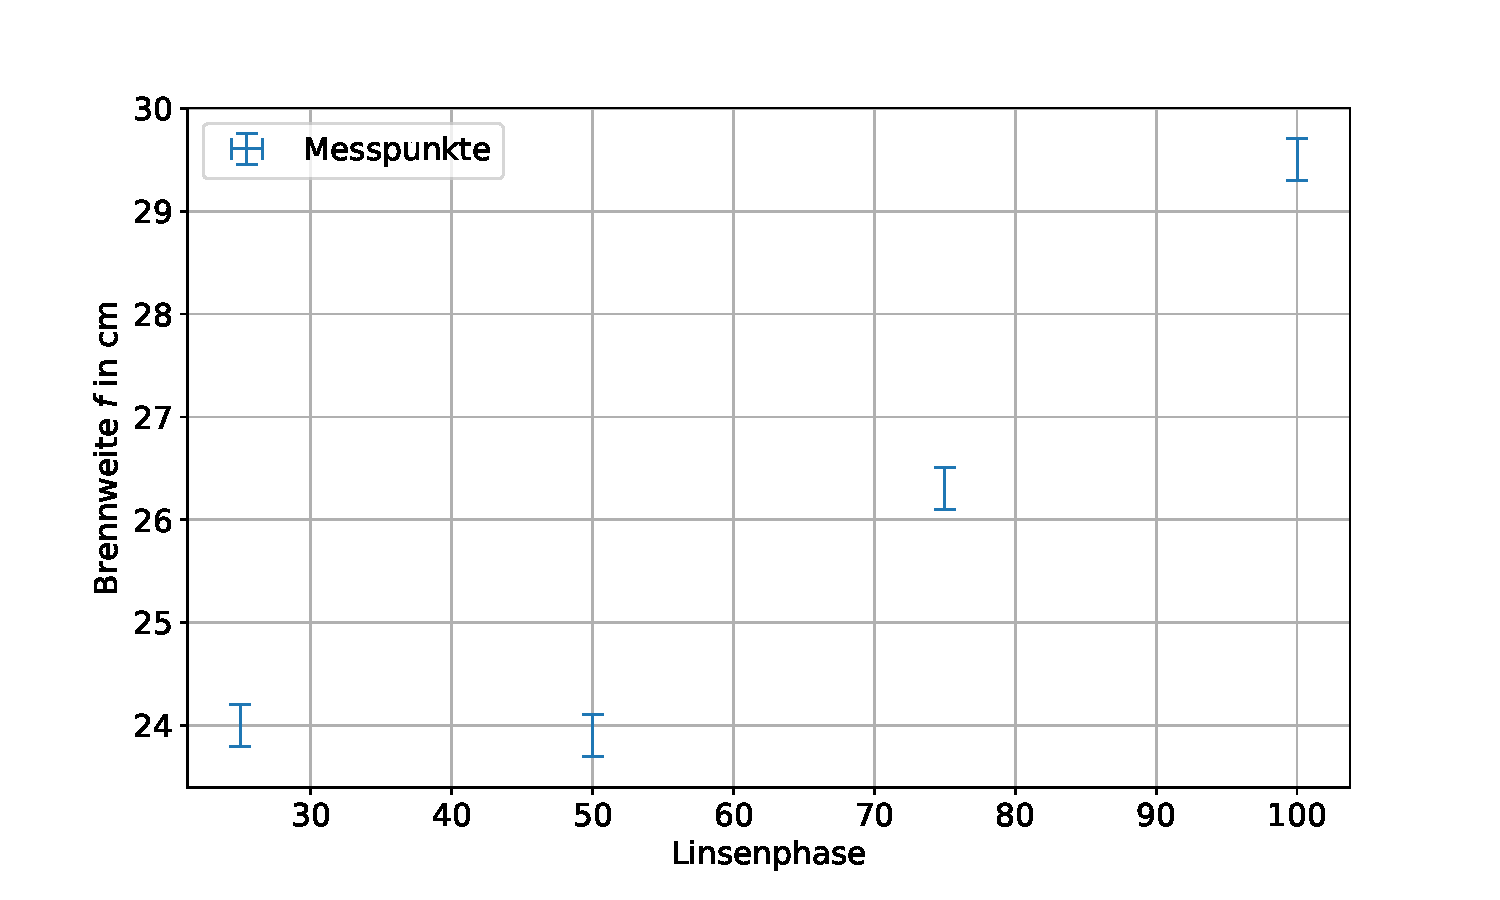
\includegraphics[width=0.8\linewidth]{img/fresnel}
			\caption{
			Die Brennweite $f$ ist gegen die Linsenphase aufgetragen.
			}
			\label{fig_fresnel}
	\end{figure}
			\subsubsection*{Diskussion}
			% die Anleitung klingt so, als würden sich da mehrere Fokuspositionen ergebn, aber das kann ja wohl nicht sein.
			% auftretende Proportionalität beschreiben
			% feststellen: Computergesteuerte Hologramme können als Linsen verschiedener Brennweite agieren.


		Wie in \cref{fig_fresnel} zu erkennen ist, nimmt die Brennweite mit der Linsenphase zu.
		In den letzten drei Messpunkten sieht der Zusammenhang linear aus, aber um über die Art der Proportionalität eine Aussage treffen zu können, wären zusätzliche Messpunkte nötig.
		Computergesteuerte Hologramme können also als Linse variabler Brennweite verwendet werden. %lol generischer Satz

		\subsection{Verschiedene DOEs als Hologramme}
		%4.3.2, 4.3.3
		% Bilder
 		\cref{fig_beug_mix} zeigt einige mit der Kamera aufgenommene Beugungsbilder mit zugehörigen Originalen.
\begin{figure}[H]
        \centering
        \begin{subfigure}[b]{0.300\textwidth}
            \centering
            
\includegraphics[width=\textwidth]{raw/holoeye_org}
            \caption%
            {Original}
            \label{fig_holoeye_org}
        \end{subfigure}
				\quad
        \begin{subfigure}[b]{0.475\textwidth}
            \centering
            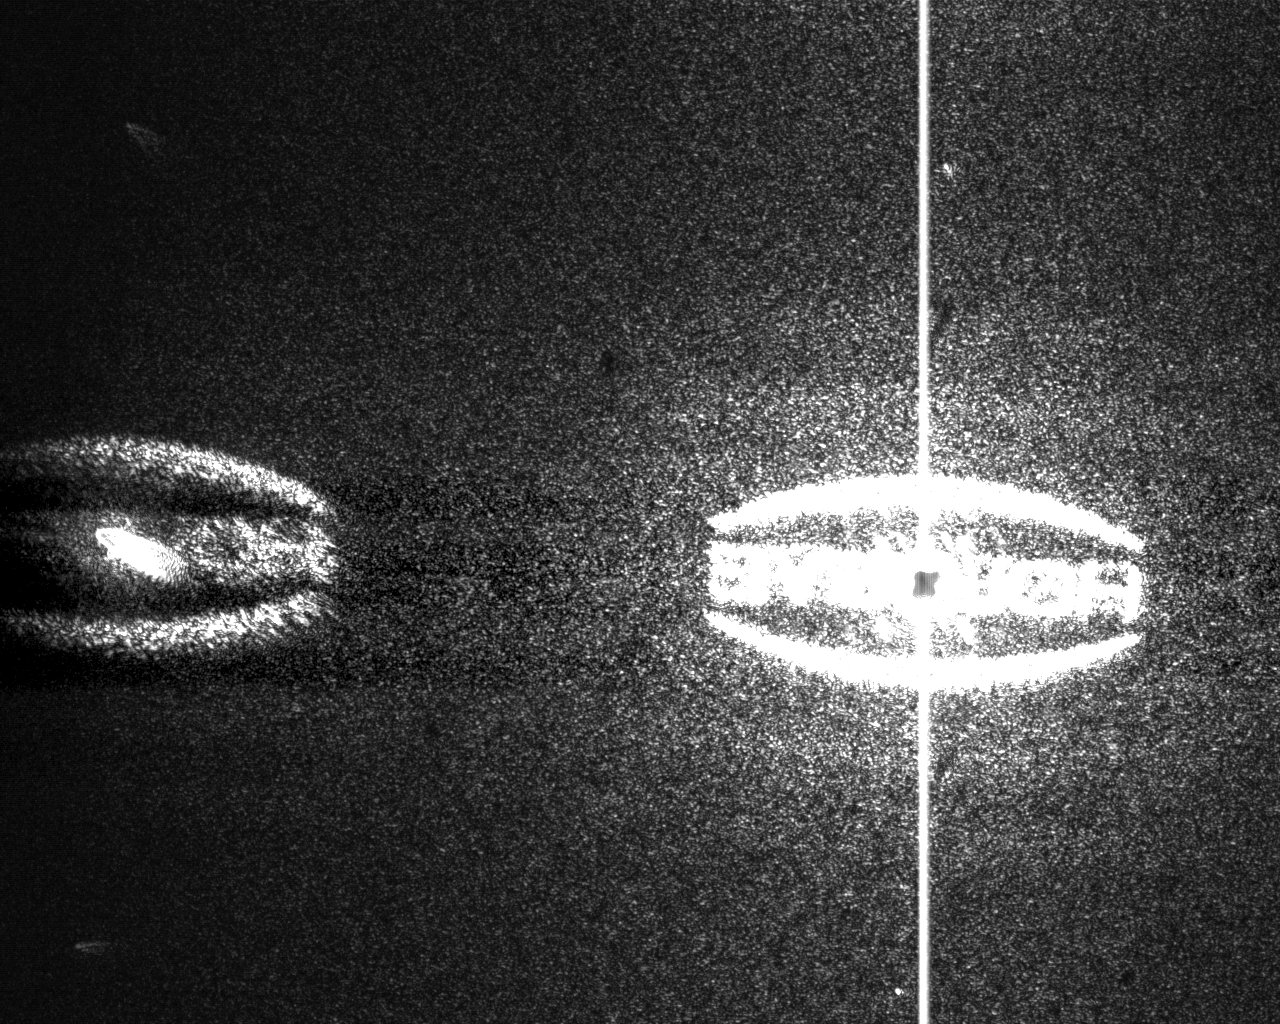
\includegraphics[width=\textwidth]{raw/holoeye}
            \caption%
            {Beugungsbild}
            \label{fig_holoeye}
        \end{subfigure}
        \vskip\baselineskip
        \begin{subfigure}[b]{0.300\textwidth}
            \centering
            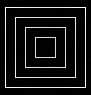
\includegraphics[width=\textwidth]{raw/square_org}
            \caption[]%
            {Original}
            \label{fig_square_org}
        \end{subfigure}
        \quad
        \begin{subfigure}[b]{0.475\textwidth}
            \centering
            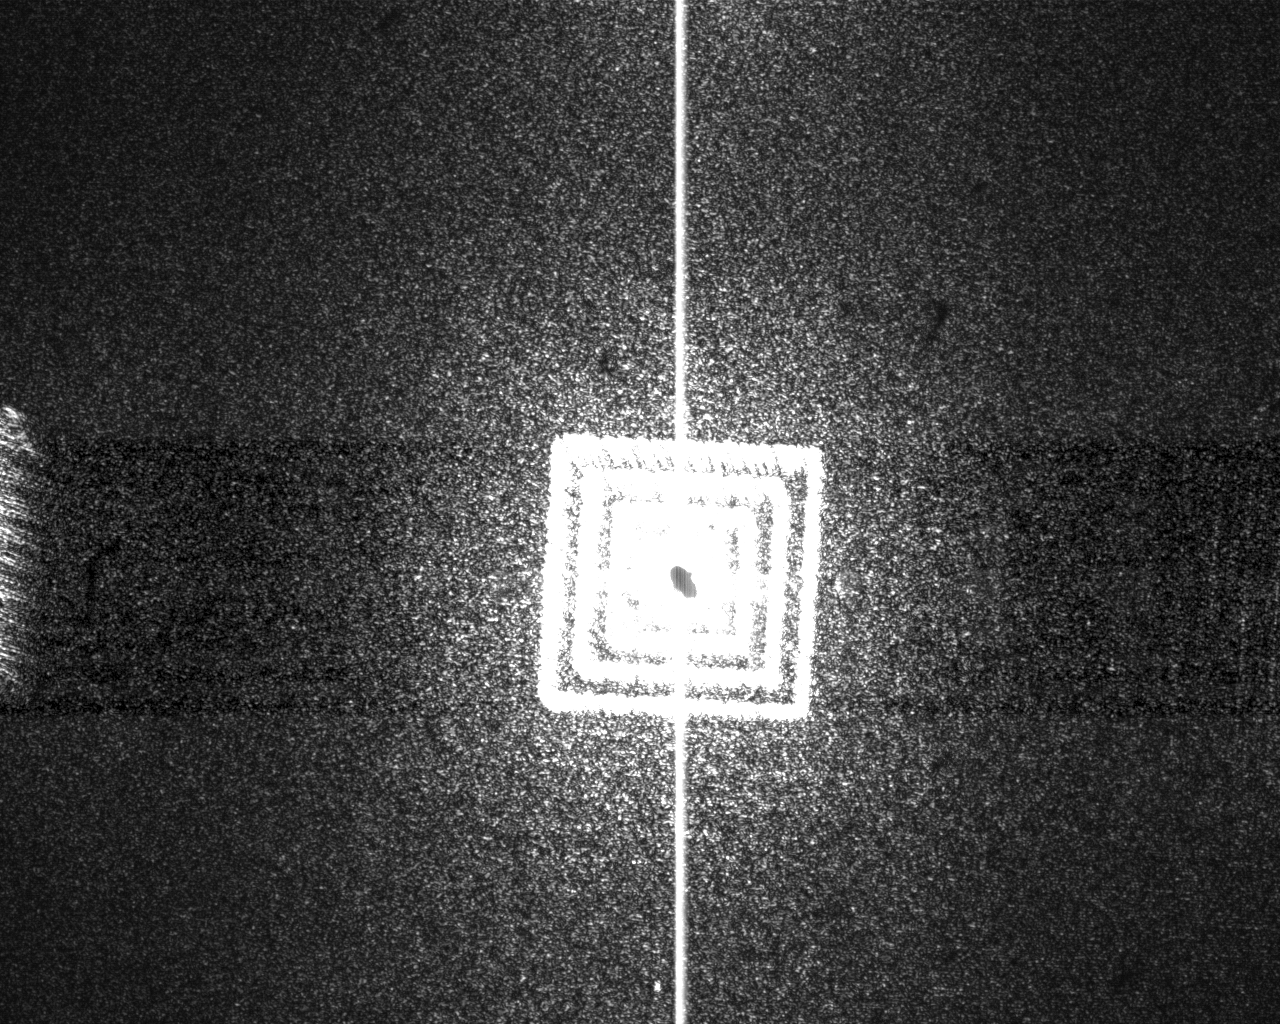
\includegraphics[width=\textwidth]{raw/square_0_ord}
            \caption[]%
            {Beugungsbild}
            \label{fig_square}
        \end{subfigure}
        \vskip\baselineskip
        \begin{subfigure}[b]{0.300\textwidth}
            \centering
            
\includegraphics[width=\textwidth]{raw/rings_org}
            \caption[]%
						{Orginal}
            \label{fig_ring_org}
        \end{subfigure}
        \quad
        \begin{subfigure}[b]{0.475\textwidth}
            \centering
            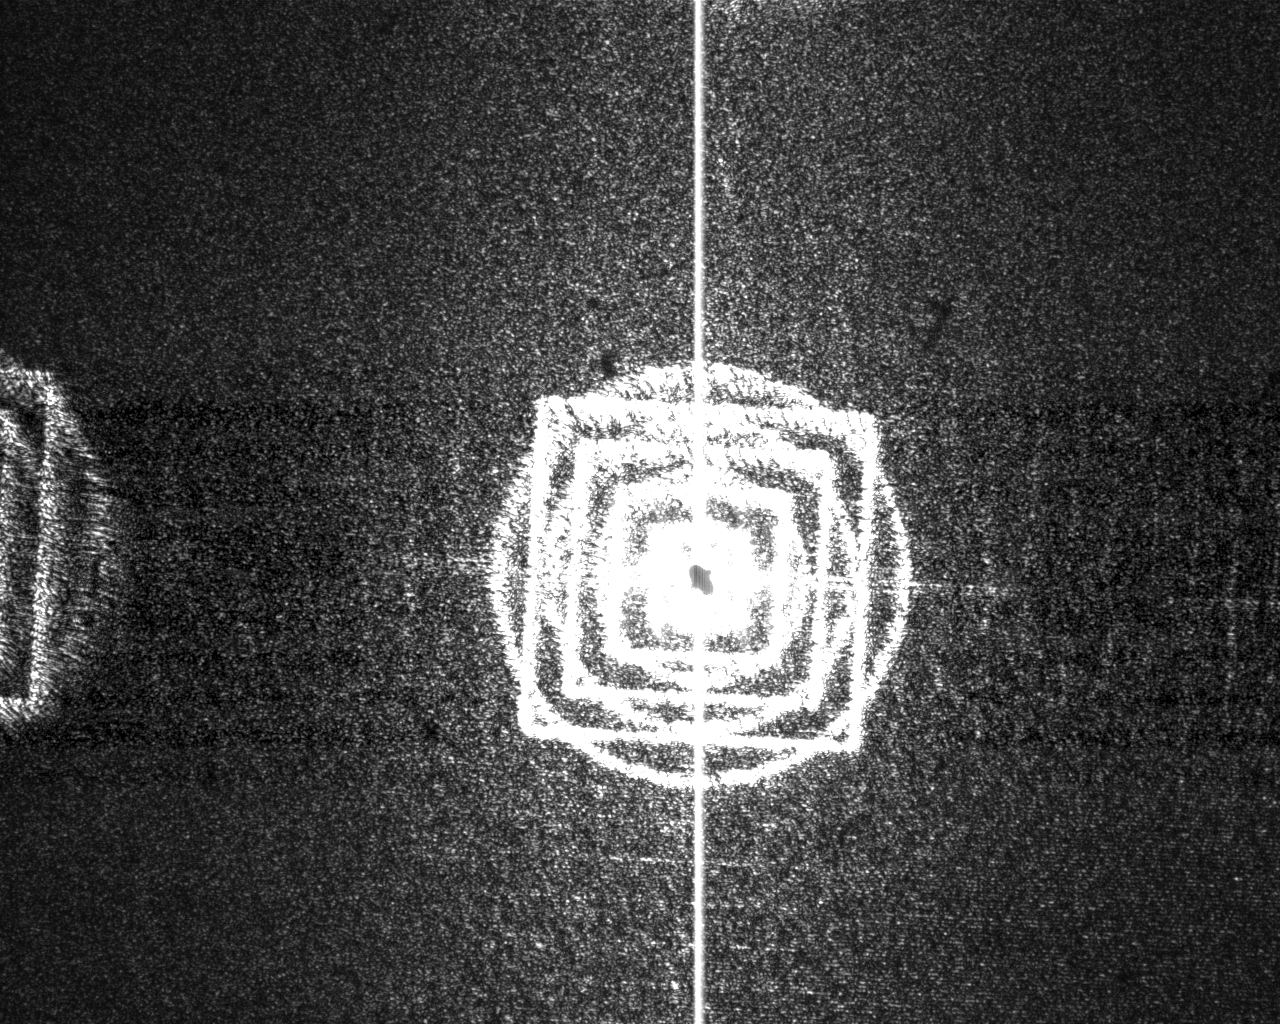
\includegraphics[width=\textwidth]{raw/square_ring_0_ord}
            \caption[]%
            {Überlagerung von \cref{fig_square_org} und \cref{fig_ring_org}}
            \label{fig_square_ring}
        \end{subfigure}
        \vskip\baselineskip
        \caption%
        {Kameraaufnahmen verschiedener Beugungsbilder im Vergleich zum Original, dass an den LC-Modulator übermittelt wird.}
        \label{fig_beug_mix}
    \end{figure}

			\subsubsection*{Diskussion}
			% DOEs nebeneinander: qualitativ Beugungsbild beschreiben, zugrundeliegenden physikalischen Effekte beschreiben
			% Glas-Hologrammfrage beantworten
			In \cref{fig_beug_mix} ist gut zu erkennen, dass durch den LC-Modulator eine Fouriertransformation stattfindet, weshalb auf dem Kamerasensor wieder das ursprüngliche Bild abgebildet wird.
			Dabei tritt aufgrund des Strahlendurchgangs durch die Modulator eine Spiegelung auf (wie durch eine Fokussierlinse).
			Das in zwei Teile getrennte Hologramm führt in \cref{fig_square_ring} zu einer Überlagerung der beiden Strukturen.
			Dies lässt sich auffassen als positive Frequenzen des einen Bildes und negative Frequenzen des anderen.
			Im Ortsraum entsteht dadurch die Überlagerung der beiden Bilder, da nicht zwischen positiven und negativen Frequenzen unterschieden wird.
			Anders gesagt beugt die eine Hälfte des LC-Modulators die Lichtstrahlen so auf den Sensor, dass Ringe entstehen und die andere so, dass Rechtecke entstehen.

			Analog dazu würde sich bei einem statisch auf eine dünne Glasplatte aufgeprägten Hologramms bei Verwendung nur einer Hälfte der Glasplatte immer noch das volle Beugungsbild ergeben und nur die Intensität verringert werden.

	\section{Schlussfolgerung}
	% Rückgriff auf Hypothese und drittes Nennen dieser

	Insgesamt gesehen lässt sich sagen, dass der verwendete LC-Modulator charakterisiert werden konnte und gezeigt werden konnte, dass er als variables DOE verwendet werden kann.
	Das Gesetz von Malus konnte bestätigt werden und die Eingangspolarisation des Modulators eingestellt werden.
	Die Pixelgröße wurde innerhalb der Messunsicherheiten in Übereinstimmung mit den Herstellerangaben bestimmt.
	Die Abhängigkeit der Ausgangspolarisation vom eingestellten Grauwert wurde untersucht und erklärt.
	Es wurden Beugungsbilder verschiedener DOEs aufgenommen und verglichen und der Modulator wurde als variable Fresnel-Linse verwendet sowie deren Brennweite in Abhängigkeit von der Linsenphase gemessen.
	Die Bestimmung der Proportionalität des Beugungswirkungsgrades zum Grauwert der Stege konnte nicht erfolgreich durchgeführt werden.
	Um hier zu einem Ergebnis zu kommen, könnte der Versuchsteil mit verschiedenen Gitterperiodizitäten durchgeführt werden.
	Zuletzt wurde der LC-Modulator verwendet, um Hologramme zu erzeugen, indem fouriertransformierte DOEs verwendet wurden.

	% Quellen zitieren, Websites mit Zugriffsdatum
	% Verweise auf das Laborbuch (sind erlaubt)
	% Tabelle + Bilder mit Beschriftung
	\printbibliography
\end{document}

%TODO Seiten fixen
